\documentclass[12pt,oneside]{memoir} 

\usepackage[latinica, biblatex]{matfmaster} 
\usepackage{listings}
\usepackage{listings-golang}
\usepackage{color}
\usepackage{tikz}
\usepackage{pgfplots}
\usetikzlibrary{pgfplots.groupplots}
\usepackage{diagbox}
\usepackage{array}
\usepackage{fancyvrb}

\definecolor{background}{RGB}{255, 248, 220}


\lstset{ 
    frame=single,
    basicstyle=\footnotesize,
    keywordstyle=\color{blue},
    showstringspaces=false, 
    stringstyle=\color{red},
    tabsize=4,
    language=Golang
}

\lstnewenvironment{snippet}[1][]
    {\lstset{float=tpb,#1}} 
    {}



\bib{literatura}


\autor{Miloš Mitrović}
\naslov{Konkurentnost u programskom jeziku Go}
\godina{2018}
\mentor{dr Milena \textsc{Vujošević Janičić}\\ Univerzitet u Beogradu, Matematički fakultet}
\komisijaA{dr Vesna \textsc{Marinković}\\  Univerzitet u Beogradu, Matematički fakultet}
\komisijaB{dr Milan \textsc{Banković}\\  Univerzitet u Beogradu, Matematički fakultet}


\apstr{
Situacija u računarstvu u današnje vreme višejezgarnih procesora, mrežnih sistema i velikih serverskih projekata koji se mogu sastojati od nekoliko desetina miliona linija koda, značajno se razlikuje od sredine u kojoj su kreirani jezici kao što su C, C++ i Python. Programski jezik Go je upravo dizajniran sa ciljem postizanja maksimalne produktivnosti u ovakvoj sredini, na takav način da programeru maksimalno olakša sam proces razvoja softvera.

Go je statički tipizirani programski jezik koji se kompilira, sa jednostavnom sintaksom koja omogućava razvoj kvalitetnog softvera sa malim brojem linija koda. Jedna od glavnih osobina koje Go čini posebnim je njegova konkurentnost koja je ugrađena u sam jezik i na intuitivan način obezbeđuje programeru pisanje memorijski i vremenski efikasnih programa sa veoma čitljivim kodom.

Rad opisuje karakteristike jezika Go, posebno istražuje njegovu konkurentnost i daje rezultate uporednih testova konkurentnog izvršavanja implementacija izabranih algoritima u jezicima Go, C, C++ i Python. Go predstavlja jezik opšte namene, ali zbog svoje dobro realizovane konkurentnosti, pogodan je za razvoj serverskih aplikacija, pa je iz tog razloga kao primer upotrebe razvijena serverska aplikacija koja demonstrira način na koji se konkurentnost može iskoristiti, kao i pojedine druge aspekte programskog jezika.
}


\kljucnereci{programski jezik Go, konkurentno programiranje, serverska aplikacija}

\begin{document}

\frontmatter
\naslovna
\komisija
\posveta{Mojoj sestri Ivoni}
\apstrakt
\tableofcontents*
\mainmatter

\chapter{Uvod}

Programski jezik Go je projekat koji razvija kompanija Google od 2007. godine. Postao je javno dostupan kao projekat otvorenog koda 2009. godine i u stalnom je razvoju. Cilj projekta je bio kreirati novi statički tipiziran jezik koji se kompilira, koji bi omogućavao jednostavno programiranje kao kod interpretiranih, dinamički tipizarnih programskih jezika. 

Smatara se da Go pripada C familiji programskih jezika, ali pozajmljuje i adaptira ideje raznih drugih jezika, izbegavajući karakteristike koje dovode do komplikovanog i nepouzdanog koda. Iako nije objektno-orijentisan, Go podržava određene koncepte kao što su metodi i interfejsi koji pružaju feleksibilnu apstrakciju podataka. Go omogućava efikasnu konkurentnost koja je ugrađena u sam jezik, kao i automatsko upravljanje memorijom, odnosno sakupljanje smeća. 

Zbog svojih osobina kao što je konkurentnost, Go je posebno dobar za izradu različitih vrsta serverskih aplikacija, ali je pre svega jezik opšte namene pa se može koristiti za rešavanje svih vrsta problema. Ima primenu u raznim oblastima kao što su grafika, mobilne aplikacije, mašinsko učenje i još mnoge druge. Osim kompanije Google, koristi se u velikom broju drugih kompanija kao alternativa jezicima poput Python-a i Javascript-a, jer pruža znatno viši stepen efikasnosti i bezbednosti.

U radu su istražene i opisane karakteristike programskog jezika Go (glava 2), sa akcentom na njegove mogućnosti za konkurentno programiranje (glava 3). Implementirana su konkurentna rešenja izabranih algoritama u programskim jezicima Go, C, C++, Python, i urađena je uporedna analiza vremenskih i memorijskih zahteva u  zavisnosti od dimenzije problema i broja jezgara na kojima se softver izvršava (glava 4). Kao primer upotrebe, razvijena je serverska aplikacija koja demonstrira korišćenje konkurentnosti kao i drugih aspekata jezika Go (glava 5).

% GO OPIS==============================================================================

\chapter{Karakteristike programskog jezika Go}

U ovoj glavi, opisane su karakteristike i osnovni koncepti programiranja jezika Go.  Konkurentnost jezika je detaljnije opisana i njoj je posvećena glava \ref{conc}.

\section{Go alat}

Alat \texttt{go} predstavalja osnovni alat za upravljanje Go kodovima. Neke od definisanih komande u okviru alata su: \texttt{build} za kompilaciju paketa, \texttt{run} za kompilaciju i izvršavanje Go programa, \texttt{test} za testiranje paketa, \texttt{get} za preuzimanje i instaliranje paketa, \texttt{fmt} za formatiranje koda paketa. Alat se upotrebljava \texttt{go komanda [argumenti]} notacijom.

\section{Početni primer}

Početni primer \textit{Hello World} u jeziku Go, prikazan je u listingu \ref{lst:hello}. Na početku programa navodi se naziv paketa. Svaki paket koji sadrži \texttt{main} funkciju, mora nositi naziv \texttt{main}. Sa \texttt{import} naredbom, navode se nazivi svih paketa koji se koriste u programu. Go ne dozvoljava importovanje suvišnih paketa, već se mogu navesti samo paketi koji se upotrebljavaju u programu. Ukoliko se navede paket koji se ne koristi, biće prijavljena greška tokom kompilacije. Nakon svake naredbe, nije obavezno navođenje znaka \texttt{;} , osim ako je potrebno navesti više naredbi u istoj liniji. 

\begin{center}
\begin{lstlisting}[caption=Hello World program u jeziku Go,label={lst:hello},  backgroundcolor=\color{background}]
package main

import "fmt"

func main() {
	fmt.Println("Hello World!")
}
\end{lstlisting}
\end{center}

\section{Tipovi podataka}

Go je statički tipiziran jezik što znači da se promenljivoj dodeljuje tip prilikom njene deklaracije i on se ne može menjati tokom izvršavanja programa. Za razliku od C-a, Go ne podržava automatsku konverziju tipova vrednosti već se konverzija vrednosti mora navesti eksplicitno, u suprotnom prijavljuje se greška prilikom kompilacije. Pravilo koje važi za pakete važi i za promenljive, svaka deklarisana promenljiva mora biti upotrebljena.

Primer prikazan u listingu \ref{lst:add} pokazuje definiciju i deklaraciju različitih vrsta promenljivih. Tip promenljive se ne mora ekspilicitno navesti, već se može zaključiti na osnovu dodele operatorom \texttt{:=} kada se promenljiva uvodi. Iako nije definisana, promenljiva \texttt{a} ima podrazumevanu vrednost koja je za numeričke tipove 0.

\begin{center}
\begin{lstlisting}[caption=Primer programa koji ilustruje rad sa promenljivama, label={lst:add},  backgroundcolor=\color{background}]
package main

import "fmt"

func main() {
	var a float32
	b := 5
	var c int

	c = int(a) + b
	fmt.Println(c)	 // 5
}
\end{lstlisting}
\end{center}

\newpage

Tipovi podataka koji su definisani u programskom jeziku Go, mogu se klasifikovati u četiri kategorije \cite{bookGoProg}: 
\begin{enumerate}
\item Bazični tipovi  (numerički, bulovski, tekstualni)
\item Složeni tipovi (nizovi i strukture)
\item Referentni tipovi (pokazivači, isečci, mape, kanali, funkcije)
\item Interfejsni tipovi (interfejsi)
\end{enumerate}


\subsection{Bazični tipovi podataka}

Bazični tipovi koji postoje u programskom jeziku Go, podeljeni su na:
\begin{itemize}

\item Numeričke -  celobrojne označene (\texttt{int8}, \texttt{int16}, \texttt{int32}, \texttt{int64}),
 celobrojne neoznačene  (\texttt{uint8}, \texttt{uint16}, \texttt{uint32}, \texttt{uint64}), u pokretnom zarezu (\texttt{float32}, \texttt{float64}) i kompleksne (\texttt{complex64}, \texttt{complex128})

\item Bulovske  (\texttt{bool})

\item Tekstualne (\texttt{string})

\end{itemize}

Konstante (\texttt{const}) u Go-u, predstavljaju izraze čija vrednost je unapred poznata kompilatoru i čija evaluacija se izvršava tokom kompilacije, a ne tokom izvršavanja programa. Konstante se mogu definisati samo za bazične tipove podataka. 

Paket strings pruža veliki broj funkcija za manipulaciju tipom \texttt{string}. Iako u okviru paketa postoji funkcija \texttt{Compare}, Go dozvoljava poređenje stringova operatorom \texttt{==}, kao i ostalim relacionimi operatorima.
\\

Operatori koji su definisani u Go-u, podeljeni su u sledeće kategorije:
\begin{itemize}

\item Aritmetički operatori ( \texttt{+} ,  \texttt{-} , \texttt{*} ,  \texttt{/} ,  \texttt{\%} ,  \texttt{++} ,   \texttt{- -} )
\item Relacioni operatori ( \texttt{==} ,  \texttt{!=} ,  \texttt{>} ,  \texttt{<} ,  \texttt{>=} ,  \texttt{<=})
\item Logički operatori (\texttt{\&\& },  \texttt{||} ,  \texttt{!})
\item Bitski operatori ( \texttt{\&} ,  \texttt{|} ,  \texttt{\^} ,  \texttt{>{}>} ,  \texttt{<{}<})
\item Operatori dodele ( \texttt{=} ,  \texttt{+=} ,  \texttt{-=} ,  \texttt{*=} ,  \texttt{/=} ,  \texttt{\%=} ,   \texttt{>{}>=} ,  \texttt{<{}<=} ,  \texttt{\&=} ,  \texttt{|=} ,  \texttt{\^{}=} )

\end{itemize}

Upotreba nad određenim tipovima podataka, uloga i arnost Go operatora, definisani su na isti način kao u jeziku C. Izuzeci su naglašeni ukoliko postoje. 

\subsection{Složeni tipovi podataka}
U složene tipove podatka u programskom jeziku Go spadaju \textbf{nizovi} i \textbf{strukture}.
\\

\textbf{Niz} predstavlja sekvencu elemenata fiksne dužine, određenog tipa podataka. Elementima niza se pristupa standardnom \texttt{[indeks]} notacijom, gde prvi element ima indeks 0. Ugrađena funkcija \texttt{len}, koristi se za dobijanje podatka o dužini niza. Dužina niza se mora navesti prilikom deklaracije ili, ukoliko se izvršava i inicijalizacija, umesto dužine, može se navesti znak \texttt{...} , a dužina će biti zaključena na osnovu incijalizacije.

Go dozvoljava poređenje nizova iste dužine definisanih nad istim tipom podataka, relacionim operatorima \texttt{==} i \texttt{!=} . Dva niza su jednaka ako imaju jednake vrednosti na istim pozicijama. U listingu \ref{lst:arr_str} je prikazan primer definisanja i upotrebe niza.
\\

\textbf{Strukture} su složeni podaci koji grupišu nula ili više elemenata proizvoljnog tipa. Svaki element mora biti jedinstveno imenovan i predstavlja jedno polje strukture. Definisanjem strukture, definiše se novi tip podataka korišćenjem ključne reči \texttt{type} ispred same definicije strukture. Poljima strukture, pristupa se pomoću znak \texttt{.} i naziva polja. Prazne strukture \texttt{struct\{\}}, mogu se koristiti za komunikaciju preko kanala u slučajevima kada nije bitan sadržaj poruke već samo davanje signala. U implementaciji \textit{quicksort} algoritma u potpoglavlju \ref{qs:go}, prikazan je primer upotrebe praznih struktura za realizaciju semafora. 

Ugnježdavanje struktura je dozvoljeno, odnosno definisanje struktura koje sadrže druge strukture kao polja. Strukture istog tipa, mogu se porediti relacionim operatorima   \texttt{==} i \texttt{!=} . Dve strukture su jednake ako imaju jednake vrednosti na istim poljima. Nad strukturama se mogu definisati metodi koji su opisani u poglavlju \ref{metod}. Primer koji demonstrira rad sa strukturama, prikazan je u listingu  \ref{lst:arr_str}.

Prilikom alociranja memorije za nizove i strukture umesto deklarisanja promenljivih, može se koristiti ugrađena funkcija \texttt{new} koja vraća pokazivač na alocirani niz ili strukturu. Nizovi se funkcijama prosleđuju kao kopija, ne preko reference kao što je slučaj u drugim jezicima poput C-a. Prenošenje niza preko reference, mora se eksplicitno naglasiti korišćenjem pokazivača. Pristupanje vrednostima niza unutar funkcije, postiže se korišćenjem operatora \texttt{*} odnosno notacijom \texttt{(*naziv)[indeks]}. Ukoliko se struktura prosledi funkciji preko reference, poljima se može pristupiti uobičajenom upotrebom znaka \texttt{.} i naziva polja.


\begin{center}
\begin{lstlisting}[caption=Primer koji demonstrira rad sa nizovima i strukturama, label={lst:arr_str},  backgroundcolor=\color{background}]
	var a [3]int
	b := [...]int{1, 2, 3}
	a[0] = 1
	fmt.Println(a==b) // false

	type Point struct{ X, Y int }
	p1 := Point{1, 2}
	p2 := Point{Y:2}
	p2.X = 1
	fmt.Println(p1==p2) // true

	c := new([3]int)
	c[0] = 1
	fmt.Println(a == *c) // true			
\end{lstlisting}
\end{center}

\subsection{Referentni tipovi podataka}
U referentne tipove podataka spadaju \textbf{pokazivači}, \textbf{isečci}, \textbf{mape}, \textbf{kanali} i \textbf{funkcije}. U ovom segementu, opisani su svi referentni tipovi podataka osim funkcija, kojima je posvećeno potpoglavlje \ref{func}, i kanala, koji su opisani u glavi \ref{conc} čija je tema konkurentnost, u poglavlju \ref{chanel}. 
\\

\textbf{Pokazivač} referiše na vrednost neke promenljive koja se trenutno čuva u memoriji. Pokazivači kao vrednost čuvaju lokaciju promenljive u memoriji na koju referišu. Za dobijanje lokacije promenljive, koristi se operator \texttt{\&}. Za dereferenciranje pokazivača, odnosno dobijanje vrednosti na koju pokazivač referiše, koristi se operator \texttt{*}.
\\

\textbf{Isečak} (eng. "slice") u programskom jeziku Go, predstavlja pogled na elemente niza. Za razliku od nizova, isečci su promenljive dužine. Svaki isečak se sastoji od tri podatka: pokazivača na niz, dužine i kapaciteta. Sintaksa za rad sa isečcima je ista kao i za rad sa nizovima, osim što prilikom deklaracije nije potrebno navoditi dužinu isečka. Za alociranje isečaka, koristiti se ugrađena funkcija \texttt{make}, koja kao parametre ima tip, dužinu i kapacitet isečka. Funkcija kreira isečak koji sadrži onoliko elemenata kolika mu je zadata dužina, koji su postavljeni na podrazumevane vrednosti. Kapacitet isečka nije fiksan, a za podatak o njegovoj trenutnoj vrednosti koristi se ugrađena funkcija \texttt{cap}.

Definisanje isečka nad nizom, postiže se korišćenjem \texttt{niz[od:do]} notacije, pri čemu se gornja granica ne uključuje. Ukoliko se donja granica izostavi, donja granica je početak niza, ukoliko se gornja granica izostavi, gornja granica je kraj niza, a ukoliko se navede samo znak \texttt{:} , isečak će sadržati sve elemente niza. 

\begin{figure}
\begin{center}
\includegraphics[scale=0.37]{slice.png}
\end{center}
\caption{Poziv funkcije \texttt{append} kada postoji i kada ne postoji dovoljno prostora za dodavanje}
\label{fig:slice}
\end{figure}

\begin{center}
\begin{lstlisting}[caption=Primer koji demonstrira rad sa isečcima, label={lst:slice},  backgroundcolor=\color{background}]
	a := [...]int{1, 2, 3, 4, 5}
	
	s1 := a[:3] 				
	fmt.Println(s1, cap(s1))	// [1 2 3] 5
	
	s1 = append(s1, 6) 			// [1 2 3 6]
	a[0] = 10					// deluje i na s1
	s2 := make([]int, 4, 4)		// [0 0 0 0] 
	copy(s2, s1)
	s1[1] = 11					// ne deluje na s2
	
	fmt.Println(s1, cap(s1)) 	// [10 11 3 6] 5
	fmt.Println(s2, cap(s2)) 	// [10 2 3 6] 4
	
	s1 = append(s1, 7, 8)		// realocira s1
	a[2] = 12					// ne deluje na s1
	fmt.Println(s1, cap(s1))	// [10 11 3 6 7 8] 12
\end{lstlisting}
\end{center}

Za rad sa isečcima postoji ugrađena funkcija \texttt{copy} koja kopira elemente jednog isečka u drugi i kao rezultat vraća broj kopiranih elemenata. Maksimalan broj elemenata koji će biti kopiran, jednak je dužini kraćeg isečka. Dozvoljeno je da isečci pre kopiranja dele elemente. Funkcija \texttt{append}, koristi se za dodavanje elemenata isečku. Tokom rada, ukoliko ne postoji dovoljno mesta, funkcija može imati potrebu da realocira niz i zbog toga kao rezultat vraća ažuriranu referencu na isečak. Nakon poziva funkcije \texttt{append}, moguće je da isečci koji su delili elemente niza, pokazuju na različite nizove, što je i prikazano na slici \ref{fig:slice} \cite{bookGoProg}. Primer koji ilustruje rad sa isečcima, prikazan je u listingu \ref{lst:slice}
\\

\textbf{Mapa} je referentni tip podataka koji referiše na heš tabelu. U tabeli se čuvaju parovi ključ - vrednost, pri čemu je vrednost svakog ključa jedinstvena. Svi ključevi su istog tipa i sve vrednosti su istog tipa. Jedini uslov je da se tip ključa može porediti operatorom \texttt{==} , dok vrednosti mogu biti proizvoljnog tipa, uključujući i druge mape. 

Funkcija \texttt{make} se koristi prilikom alociranja prostora za novu mapu. Upis u mapu, postiiže se \texttt{naziv[ključ] = vrednost} notacijom. Ugrađena funkcija \texttt{delete}, koristi se za brisanje parova iz mape. Kao parametre, funkcija ima naziv mape i ključ para koji se briše. Ukoliko ključ ne postoji, funkcija nema nikakav efekat. Dodeljivanje vrednosti promenljivoj na osnovu ključa iz mape, postiže se \texttt{v := naziv[ključ]} notacijom, pri čemu, ukoliko ključ ne postoji, vrednost \texttt{v} će biti postavljena na podrazumevanu. Moguće je izvršiti proveru da li je određeni ključ definisan u mapi, upotrebom \texttt{v, ok := naziv[ključ]} ili  \texttt{\_, ok := naziv[ključ]} notacije, gde je \texttt{ok} promenljiva tipa \texttt{bool}, koja je nosi informaciju da li ključ postoji ili ne. 

U programskom jeziku Go, operacije nad mapama nisu atomične i prilikom konkurentnog korišćenja, potrebno je koristiti odgovarajuće mere sigurnosti koje su opisane u glavi \ref{conc}. Primer koji demonstrira rad sa mapama, prikazan je u listingu \ref{lst:map}.

\begin{center}
\begin{lstlisting}[caption=Primer koji demonstrira rad sa mapama, label={lst:map},  backgroundcolor=\color{background}]
	m1 := make(map[string]int)
	m1["a"] = 1
	m2 := map[string]float32{"m": 1.23, "a": 2.34}
	
	_, ok := m2["b"]
	delete(m2, "p")		// nema efekta
	delete(m2, "a")
	fmt.Println(m2, ok) // [m:1.23] false
\end{lstlisting}
\end{center}

\section{Kontrole toka}

U programskom jeziku Go, naredbe za kontrolu toka izvršavanja su \texttt{if}, \texttt{switch}, \texttt{for} i \texttt{defer}. Naredba \texttt{if}, ponaša se na isti način kao i u drugim jezicima i omogućava standardnu \texttt{if, else if, else} strukturu. Pre uslova, moguće je navesti jednu naredbu koja je razdvojena sa znakom\texttt{;} od uslova. 

Naredba \texttt{switch} omogućava ispitivanje uslova po slučajevima upotrebom \texttt{switch case default} stukture. Ukoliko je uslov za neki slučaj (\texttt{case}) zadovoljen, izvršiće se deo koda naveden nakon znaka \texttt{:} , do definicije seledećeg slučaja ili kraja naredbe, u suprotnom izvršava se \texttt{default} slučaj. Ukoliko se na kraju slučaja navede \texttt{fallthrough} naredba, izvršava se i k\^{o}d slučaja direktno ispod. Za pojedinačni slučaj moguće je navodti više uslova razdvojenim zarezima. 

Jedina petlja koja postoji u programskom jeziku Go jeste \texttt{for}. Petlja ima standardnu trodelnu strukturu razdvojenu znakom \texttt{;} , gde se prvi deo  izvršava samo jedanput na početku, drugi deo predstavlja uslov koji se proverava na početku svake iteracije a treći deo predstavlja inkrementalni korak koji se izvršava na kraju svake iteracije. Za izlazak iz petlje, koristi se \texttt{break} naredba, a naredba \texttt{continue} za prelazak na sledeću iteraciju. \texttt{For} petlja se može koristiti zajedno sa \texttt{range} naredbom za iteriranje kroz sekvencijalne strukture kao što su nizovi, isečci i mape. 

\begin{center}
\begin{lstlisting}[caption=Primer koji demonstrira upotrebu kontrolnih struktura, label={lst:control},  backgroundcolor=\color{background}]
	a := [...]uint{1, 2, 3}
	if len(a) > 1 {
		for i,v := range a {	
			fmt.Println(i,v) // indeks, vrednost
		}
	}

	switch a[2] {
    case 3:
        fmt.Println("bigger than two")
		fallthrough
    case 2:
        fmt.Println("bigger than one")
    default:
        fmt.Println("one")
    }
\end{lstlisting}
\end{center}

Naredba \texttt{defer} odlaže izvršavanje navedene funkcije do trenutka završetka funkcije u kojoj se nalazi. Argumenti funkcije se određuju u trenutku navođenja \texttt{defer} naredbe, samo je izvršavanje funkcije odloženo. Naredba garantuje da će se funkcija izvršiti i u slučaju dolaska do greške. Najčešća upotreba \texttt{defer} naredbe je za operacije koje se obavljaju u paru, kao što je otvaranje i zatvaranje fajlova. Odmah nakon otvaranja fajla, moguće je \texttt{defer} naredbom pozvati funkciju za zatvaranje fajla, što osigurava da će se fajl zatvoriti i doprinosi čitljivijem kodu. 

Naredbe \texttt{if} i \texttt{for} zahtevaju upotrebu vitičastih zagrada i u slučajevima kada se u bloku nalazi samo jedna naredba, a uslove nije potrebno navoditi unutar zagrada. Primer koji ilustruje upotrebu standardnih kontrolnih struktura prikazan je u listingu \ref{lst:control}. 

Osim navedenih kontrolni struktura, Go podržava i \texttt{go to} naredbe u kombinaciji sa labelama. Generalno, upotreba \texttt{go to} naredbi nije preporučena jer dovodi do loše strukture i nečitljivog koda.


\section{Funkcije} \label{func}

Funkcije u programskom jeziku Go, predstavljaju referentni tip podataka. Sintaksa za definisanje funkcije, prikazana je u listingu \ref{lst:funcDef}.

\begin{center}
\begin{lstlisting}[caption=Sintaksa za definisanje funkcije, label={lst:funcDef},  backgroundcolor=\color{background}]
func naziv(lista parametara) (lista rezultata) {
	telo funkcije 
} 
\end{lstlisting}
\end{center}

 Osim što mogu imati proizvoljan broj argumenata, funkcije mogu imati više povratnih vrednosti. Postoje i varijadičke funkcije, odnosno funkcije sa promenljivim brojem argumenata. Varijadičke funkcije se definišu upotrebom znaka \texttt{...} ispred tipa argumenta koji se može pojaviti nula ili više puta. 

Omogućeno je definisanje funkcija unutar funkcija, gde unutrašnja funkcija ima pristup svim promenljivama spoljašnje funkcije, kao i  definisanje anonimnih funkcija, odnosno funkcija bez imena koje se izvršavaju na mestu gde su definisane. Funkcije predstavljaju tipove prvog reda i mogu se prosleđivati drugim funkcijama i dodeljivati promenljivama. Primer rada sa funkcijama, prikazan je u listingu \ref{lst:func}.

\begin{center}
\begin{lstlisting}[caption=Primer koji demonstrira rad sa funkcijama, label={lst:func},  backgroundcolor=\color{background}]
func add(args ...int) int {
	sum := 0
	for _, v := range args {
		sum += v
	}
	return sum
}
func calc(x, y int) (int, int) {
	add := func() int { return x + y }
	sub := func() int { return x - y }

	return add(), sub()
}	
func power(x int) func(int)int {
	res := 1
	return func(a int)int {
		for i:=0; i<a; i++ {
			res *= x
		}
		return res
	}
}

func main() {
	fmt.Println(add(1,2,3))		// 6
	fmt.Println(calc(1,2)) 		// 3, -1
	fmt.Println(power(2)(4))	//16
}
\end{lstlisting}
\end{center}

\section{Metodi}  \label{metod}

U programskom jeziku Go ne postoji pojam klase, ali je omogućeno definisanje metoda nad korisnički definisanim tipovima. Metod predstavlja običnu funkciju koja u sebi sadrži specijalni prijemnik (eng "receiver") za tip podataka nad kojim je metod definisan. Metod se definiše na isti način kao i funkcija, osim što se prijemnik navodi između ključne reči \texttt{func} i naziva metoda.

Pozivanje metoda, postiže se navođenjem znaka \texttt{.} i naziva metoda nakon promenljive za koju je potrebno pozvati metod. Ukoliko metod menja podatke promenljive nad kojom je pozvan, potrebno je koristiti prijemnik sa referencom. 
 
Go nema definisane nivoe vidljivosti  pomoću ključnih reči kao što su \texttt{public}, \texttt{private} i \texttt{protected}. Jedini mehanizam za kontrolu vidljivosti je sledeći: svi identifikatori koji počinju velikom slovom, biće eksportovani van paketa, svi identifikatori koji počinju malim slovom, neće biti eksportovani van paketa \cite{bookGoProg}. Isto pravilo važi i za polja strukture. Na taj način struktrure nad kojima su definisani metodi mogu da oponašaju klase i enkapsulaciju podataka. Primer koji demonstrira rad sa metodima, prikazan je u listingu \ref{lst:metod}.

\begin{center}
\begin{lstlisting}[caption=Primer koji demonstrira rad sa metodima, label={lst:metod},  backgroundcolor=\color{background}]
type Point struct{ X, Y float64 }

func (p Point) Distance(q Point) float64 {
	return math.Sqrt((p.X-q.X)*(p.X-q.X)+(p.Y-q.Y)*(p.Y-q.Y))
}

func (p *Point) Translate(x, y float64) {
	p.X += x
	p.Y += y
}

func main() {
	p1 := Point{0,0}
	p2 := Point{1,1}

	fmt.Println(p1.Distance(p2)) // 1.41421...
	p2.Translate(5,2)
	fmt.Println(p2)				// {6 3}
}
\end{lstlisting}
\end{center}

\section{Interfejsi}

Interfejsi se koriste kao dodatno sredstvo apstrakcije i enkapsulacije podataka. Tip interfejs, definisan je kao skup potpisa metoda. Svaki interfejs se sastoji od vrednosti i konkretnog tipa. Vrednost tipa interfejs, može biti bilo koja vrednost čiji tip implentira zadate metode. Konkretni tipovi su svi tipovi podataka osim interfejsa.

Tip zadovoljava neki interfejs ukoliko implementira sve metode koje taj interfejs zahteva. Unutar interfejsa, moguće je navoditi i nazive drugih interfejsa, koji takođe moraju biti zadovoljeni. Svi tipovi zadovoljavaju prazan interfejs (\texttt{interface\{\}}). Mnogi paketi i funkcije koriste interfejse, kao što je već viđeni paket \texttt{fmt} sa interfejsom \texttt{Stringer} koji se koristi za definisanje ispisa određenog tipa podataka. Greške, koje su opisane poglavlju \ref{error}, takođe predstavljaju interfejs. Primer koji demonstrira rad sa interfejsima, prikazan je u listingu \ref{lst:inter}.

\begin{center}
\begin{lstlisting}[caption=Primer koji demonstrira rad sa interfejsima, label={lst:inter},  backgroundcolor=\color{background}]
type geometry interface { 
	area() float64 
}
type rect struct {width, height float64}
type circle struct {radius float64}

func (r rect) area() float64 {
	return r.width * r.height
}
func (c circle) area() float64 {
	return math.Pi * c.radius * c.radius
}
func measure(g geometry) {
	fmt.Println(g, g.area(), g.perim())
}

func main(){
	r := rect{width: 3, height: 4}	
	c := circle{radius: 5}			
	measure(r)	//{3 4} 12 
  	measure(c)	//{5} 78.5398 
}
\end{lstlisting}
\end{center}

Pretpostavljanje tipova (eng. "type assertion") omogućava pristup konkretnom tipu u okviru interfejsa, što se postiže sa \texttt{i.(T)}, gde je i promenljiva tipa interfejs, a \texttt{T} naziv konkretnog tipa. Ukoliko se pretpostavi pogrešan tip, dolazi do greške.  Za proveru da li interfejs sadrži određeni tip, prilikom pretpostavljanja mogu se vratiti dve vrednosti, vrednost tipa i \texttt{bool} vrednost koja sadrži informaciju da li je pretpostavljanje uspešno. Za obradu pojedinačnih slučajeva za svaki od mogućih tipova može se koristiti naredba \texttt{switch}.  Primer koji demonstrira pretpostavljanje tipova, prikazan je u listingu \ref{lst:type}.

\begin{center}
\begin{lstlisting}[caption=Primer koji demonstrira pretpostavljanje tipova kod interfejsa, label={lst:type},  backgroundcolor=\color{background}]
	var i interface{} = "hello"

	s := i.(string)
	fmt.Println(s) 		// hello

	s, ok := i.(string)
	fmt.Println(s, ok) 	// hello true

	f, ok := i.(float64)
	fmt.Println(f, ok) 	// 0 false
\end{lstlisting}
\end{center}


\section{Refleksija}

U računarstvu, refleksija predstavlja sposobnost programa da izvrši ispitivanje svoje strukture i ponašanja u toku izvršavanja. Refleksija se može koristiti za ispitivanje tipova promenljivih tokom izvršavanja, u zavisnosti od čega program može da preduzme odgovarajuće akcije. Go podržava refleksiju tipova koja je omogućena upotrebom paketa \texttt{reflect}.

Unutar paketa, definisani su tipovi \texttt{Type} i \texttt{Value}, funkcija \texttt{TypeOf} za dobijanje informacije o tipu promenljive i funkcija \texttt{ValueOf} za dobijanje vrednosti promenljive. Funkcije kao argument prihvataju tip \texttt{interface\{\}}. 

Za postavljanje vrednosti, postoje \texttt{Set} metodi za svaki tip podataka koji se poziva nad tipom \texttt{Value}, kao i metod \texttt{CanSet} za proveru da li je moguće postaviti vrednost datoj promenljivi. Vrednost je moguće postaviti samo referentnim tipovima, odnosno promeniti vrednost na koju oni referišu. \texttt{Set} metodi se ne mogu pozivati nad promenljivom \texttt{Value} bez pripreme, već je nad njom prvo potrebno pozvati metod \texttt{Elem} koji omogućava pristup vrednosti na koju promenljiva referiše.  

Primer koji demonstrira osnovnu upotrebu refleksije, prikazan je u listingu \ref{lst:ref}. Paket nudi još veliki broj drugih funkcija za refleksiju tipova i njihovu manipulaciju \cite{reflect}.

Refleksija predstavlja jak alat ukoliko se upotrebljava na pravi način, ali trebalo bi je koristiti sa oprezom. Postoji nekoliko razloga za opreznost: mogućnost dolaska do greške u toku izvršavanja programa koja bi mogla biti prijavljena tokom kompilacije ukoliko program ne bi koristio refleksiju; smanjena čitljivost koda ukoliko program previše koristi refleksiju; sporije izvršavanje funkcija koje koriste refleksiju, naspram funkcija specijalizovanih za pojedinačne tipove \cite{bookGoProg}.

 \begin{center}
\begin{lstlisting}[caption=Primer koji demonstrira osnovnu upotrebu refleksije, label={lst:ref},  backgroundcolor=\color{background}]
	var x float64 = 3.14
	v := reflect.ValueOf(&x) 
	
	fmt.Println(v.Type())	// *float64
	fmt.Println(v.CanSet())	// false
	
	v = v.Elem()
	fmt.Println(v.CanSet())	// true
	
	v.SetFloat(3.15)
	fmt.Println(x)			// 3.15
\end{lstlisting}
\end{center}

\section{Upravljanje greškama} \label{error}

Stanje greške u programskom jeziku Go, označava se \texttt{error} vrednostima. Tip \texttt{error} predstavlja ugrađeni interfejs koji zahteva implementiranje \texttt{Error} metoda koji kao rezultat vraća \texttt{string} sa informacijom o grešci. Ako neka funkcija kao rezultat vraća tip \texttt{error}, njegova vrednost će biti \texttt{nil} ukoliko nije došlo do greške. 

Implementacijom \texttt{Error} metoda za neki tip, moguće je definisati novi tip greške. Ukoliko se upotrebljava već postojeći tip \texttt{error}, za definisanje poruke greške koristi se funkcija \texttt{New} iz paketa \texttt{errors}. Primer koji demonstrira upravljanje greškama, prikazan je u listingu \ref{lst:error}.

Na ovaj način omogućeno je elegantno upravljanje greškama. Funkcija \texttt{panic} je ugrađena funkcija koja se koristi za prekidanje toka izvršavanja u slučaju ozbiljnijih grešaka i nepredviđenih situacija. Ukoliko funkcija F pozove funkciju \texttt{panic}, njeno izvršavanje se prekida, a zatim se izvršavaju \texttt{defer} pozivi funkcija nakon čega se funkcija F vraća svom pozivaocu. Tada se za pozivaoca, funkcija F ponaša kao poziv funkcije \texttt{panic} i proces se ponavlja dokle god sve funkcije u tekućoj gorutini ne prestanu sa radom i dok program ne pukne. Ugrađene funkcije obično pozivaju \texttt{panic} ukoliko dođe do neke nepredviđene greške ili situacije koja se nije mogla otkriti tokom faze kompilacije, ali moguće je pozvati funkciju i manuelno. 

Pored funkcije \texttt{panic}, postoji i ugrađena funkcija \texttt{recover} koji služi za preuzimanje kontrole gorutine koje je u stanju \texttt{panic}. Funkciju \texttt{recover}, ima jedino smisla koristiti unutar \texttt{defer} nardbe. Ukoliko je tekuća gorutina u stanju \texttt{panic}, \texttt{recover} funkcija će preuzeti vrednost koju je dobila funkcija \texttt{panic} i nastaviti normalno izvršavanje programa.

\begin{center}
\begin{lstlisting}[caption=Primer koji demonstrira upravljanje greškama, label={lst:error},  backgroundcolor=\color{background}]
//definisanje novog tipa
type MyError struct {
	When time.Time
	What string
}
func (e MyError) Error() string {
	return fmt.Sprintf("%v: %v", e.When, e.What)
}
//funkcija koja koristi novi tip
func divide1(a,b float64) (float64, error) {
	if b == 0 {
		return 0, &MyError{time.Now(),"division by zero"}
	}else {
		return a/b, nil
	}
}
//funkcija koja koristi error tip
func divide2(a,b float64) (float64, error) {
	if b == 0 {
		return 0, errors.New("Division by zero")
	}else {
		return a/b, nil
	}
}
//provera greske u funkciji main
func main() {
	if v1, err := divide1(3.14,0); err != nil {
		fmt.Println(err)				
	}
	if v2, err := divide2(3.14,0); err != nil {
		fmt.Println(err)			
	}
}
\end{lstlisting}
\end{center}
 
\section{Sakupljanje smeća}

Programski jezik Go ima automatsko upravljanje memorijom odnosno sakupljanje smeća (eng. "garbage collection"). Sakupljač skenira memoriju, pronalazi objekte na koje više ne postoji ni jedna referenca i nakon toga ih briše i oslobađa memoriju. Upotrebom paketa \texttt{runtime}, sakupljač se može eksplicitno pozvati korišćenjem \texttt{GC} funkcije. 

Od verzije Go 1.5, sakupljač smeća \cite{garbage} je kreiran da bude konkurentni, trobojni, označi-počisti (eng. "mark-sweep") sakupljač. Kod trobojnih sakupljača, svaki objekat je bele, sive ili crne boje i hip se posmatra kao jedan povezani graf. Na početku ciklusa, svi objekti su beli. Sakuplač prvo posećuje sve korene grafa koji predstavljaju objekte kojima se može pristupiti direktno iz aplikacije, kao što su globalne promenljive i promenljive na steku, koje boji u sivo. Nakon toga, skaupljač bira neki od sivih objekata, boji ga u crno i proverava da li poseduje pokazivače ka drugim objektima. Ukoliko pronađe pokazivač ka belom objektu, označava ga sivom bojom. Proces se ponavlja dokle god postoje sivi objekti. Na kraju, belom bojom su označeni objekti do kojih nije moguće doći, odnosno objekti na koje niko ne referiše.

\begin{figure}
\begin{center}
\includegraphics[scale=0.33]{tricolor.png}
\end{center}
\caption{Prikaz označavanja objekata kod trobojnog algoritma}
\label{fig:tricolor}
\end{figure}

Čitav ovaj proces, izvršava se konkurentno sa aplikacijom, koja se još naziva i mutator jer menja pokazivače dok je sakupljač aktivan. Mutator ne sme da narušava pravilo da nijedan crni objekat ne pokazuje na beli, kako sakupljač ne bi izgubio evidenciju objekata koji su ubačeni u deo hipa koji je već posetio. Za očuvanje ovog pravila, zadužena je barijera za pisanje (eng. "write barrier") koja predstavlja funkciju koja se aktivira prilikom promene pokazivača na hipu. Barijera označava beli objekat kao sivi ukoliko u tom trenutku postoji neki pokazivač koji pokazuje na njega, čime se osigurava da će ga pre ili kasnije sakupljač obraditi, odnosno proveriti da li poseduje pokazivače ka drugim objektima. Šematski prikaz trobojnog algoritma, prikazan je na slici \ref{fig:tricolor}.

Sakupljač obavlja što veći deo posla konkurentno, međutim potrebno je na kratko da zaustavi sve (eng "stop the world") kako bi proverio potencijalne izvore sivih objekata. Pronalaženje pravog trenutka za zaustavljanje i njegovo samo trajanje, poboljšava se svakom novom distribucijom jezika Go. Od verzije Go 1.8, pauze uobičajeno traju manje od 100 mikrosekundi, a često se dešava da je njihovo trajanje samo 10 mikrosekundi, što je značajno unapređenje od verzije Go 1.5 gde su pauze trajale nekoliko milisekundi.

\section{Testiranje}

Programski jezik Go ima ugrađenu podršku za automatsko testiranje paketa. Testiranje se izvršava pomoću \texttt{go test} alata i \texttt{testing} paketa. Alat se koristi za testiranje funkcija i kao rezultat daje vrednosti \texttt{PASS} ili \texttt{FAIL}. Benčmark funkcije za testiranje performansi su takođe podržane. Sa alatom dolazi veliki broj flegova koji omogućava različite opcije kao što su broj ponavljanja benčmark testova ili broj korišćenih procesora prilikom testiranja. Testovi se izdvajaju u poseban test fajl. 

Funkcije za testiranje u nazvu imaju prefiks \texttt{Test}, a zatim naziv funkcije koju testiraju. Kao argument, funkcije imaju parametar \texttt{T} koji se koristi za obaveštavanje o neuspešnim testovima i logovanje dodatnih informacija. Benčmark funkcije imaju prefiks \texttt{Benchmark}, a kao argument imaju parametar \texttt{B} koji poseduje veliki broj istih metoda kao i parametar \texttt{T}, sa dodatnim stavkama koje su potrebne za merenje performansi kao što je polje \texttt{N} koje označava broj ponavljanja operacije koja se testira.

Alat \texttt{go test} takođe podržava i funkcije primere (eng. "example functions") čija je primarna uloga dokumentacija koda. Funkcije primeri imaju prefiks  \texttt{Example}, a kao argument nemaju nikakve parametre i ne vraćaju nikakav rezultat. Alat prevodi i izvršava ove funkcije, a ukoliko imaju neki ispis, on se ispisuje na standardnom izlazu. Pod komentarom koji počinje sa \texttt{Output:} , moguće je navesti ispis funkcije koji će biti upoređen sa ispisom funkcije na standardnom izlazu. Primer funkcija za testiranje, prikazan je u listingu \ref{lst:test}.

\begin{center}
\begin{lstlisting}[caption=Primer različitih tipova funkcija za testiranje, label={lst:test},  backgroundcolor=\color{background}]
// funkcija koja se testira
func Sum(x int, y int) int {  
	return x + y
}
// funkcija za testiranje
func TestSum(t *testing.T) {  
	total := Sum(1, 2)
	if total != 3 {
		t.Errorf("Sum was incorrect, got: %d, want: %d.", total, 3)
	}
}
// benchmark funkcija
func BenchmarkSum(b *testing.B) {
	for i := 0; i < b.N; i++ {
		Sum(2,2)
	}
}
// example funkcija
func ExampleSum() {
	fmt.Println(Sum(5,0))
	fmt.Println(Sum(1,3))
	// Output:
	// 5
	// 4
}

\end{lstlisting}
\end{center}

\section{Paketi}

U okviru same distribucije programskog jezika Go, postoji veliki broj paketa standardne biblioteke koji obezbeđuju različite usluge. Neki od osnovnih paketa su upotrebljeni u primerima: \texttt{fmt} za formatirani ulaz/izlaz; \texttt{strings} za rad sa stringovima; \texttt{math} sa implementacijama matematičkih funkcija. Još jedan paket koji se često upotrebljava je \texttt{os} paket koji predstavlja interfejs ka operativnom sistemu i omogućava funkcionalnosti kao što su rad sa fajl sistemom, pristup argumentima komandne linije i pokretanje procesa.

U standardnoj biblioteci, takođe postoje paketi za rad sa SQL bazama podataka, kriptografskim funkcijama, kompresiju podataka, rad sa slikama,  podršku za mrežno programiranje i još mnogi drugi. Pored paketa standardne biblioteke, postoje dodatni i prošireni paketi u okviru Go projekta koji imaju labavije uslove kompatibilnosti Go verzija. Ovde se mogu pronaći paketi za razvoj aplikacija za mobilne platforme, eksperimentalni debager, prošireni kriptografski i mrežni paketi. 

Paketi van distribucije samog jezika, mogu se preuzeti korišćenjem \texttt{go get} komande i navođenja repozitorijuma u kome se paket nalazi. Na veb sajtu \url{https://godoc.org/} mogu se naći paketi i njihove dokumentacije koje razvijaju članovi Go zajednice koja vremenom postaje sve veća. Paketi su odobreni od strane Go projekta i mogu se naći paketi koji obezbeđuju najrazličitije alate za programiranje kao i API-je mnogih postojećih servisa.


% KONKURENTNO==============================================================================
\chapter{Konkurentno programiranje u jeziku Go} \label{conc}

U ovoj glavi, objašnjeni su osnovni pojmovi i problemi koji se javljaju kod konkurentnog programiranja. Nakon toga, opisano je kako je konkurentnost realizovana u programskom jeziku Go, kako se ona upotrebljava i načini na koji se rešavaju određeni problemi. 

\section{Osnovni pojmovi konkurentnog programiranja}

U računarstvu, konkurentnost označava mogućnost procesa da određene delove izvršava nezavisno jedne od drugih, bez uticanja na sam rezultat programa. Pojam konkurentnosti se često poistovećuje sa paralelizmom. Za razliku od konkurentnosti, paralelizam podrazumeva da se delovi jednog procesa izvršavaju istovremeno, dok konkurentnost samo definiše celine koje se mogu izvršavati u preklapajućim vremenskim intervalima, ali ne obavezno istovremeno. 

\subsection{Niti}

Osnovni pojam u konkurentnom programiranju predstavlja nit. Niti su osnovne jedinice za izvršavanje u okviru procesa. Jedan proces se može sastojati od više niti koje se izvršavaju konkurentno. Niti jednog procesa dele određene resurse kao što su k\^{o}d segement i segement podataka, ali poseduju i sopstvene resurse kao što je stek. 

Korišćenje niti donosi mnoge prednosti kao što su ušteda memorijskog prostora i vremena. Niti zauzimaju manje prostora nego pojedinačni procesi jer dele određene resurse i kao rezultat se kreiraju znatno brže od procesa. Takođe, niti omogućavaju aplikacijma da obavljaju druge, nezavisne zadatke dok su neki delovi blokirani ili zauzeti. Serverske aplikacije često koriste kreiranje niti umesto kreiranja procesa za svakog novog korisnika jer se niti brže kreiraju i zauzimaju manje prostora, pa je omogućeno da se brže odgovori na zahteve i opsluži veći broj korisnika \cite{os}.  

\subsection{Problemi}

Osim prednosti koje konkurentnost donosi, postoje problemi koji se mogu javiti pri manipulaciji zajedničkih podataka i resursa. Nekontrolisano pristupanje zajedničkim podacima može dovesto do neispravnih rezultata. Ukoliko su neki resursi deljeni, kao na primer standardni izlaz, nesinhronizovani ispis može proizvesti ispreplitane, nečitljive poruke. Situacija u kojoj krajnji rezultat zavisi od redosleda izvršavanja koraka različitih procesa ili niti koji manipulišu zajedničkim podacima ili resursima naziva se trka za resurse (eng. "race condition") \cite{os}.

Na slici \ref{fig:race} levo, prikazan je jednostavan primer u kome se javlja problem trke za resurse. Problem se javlja jer uvećanje vrednosti deljene promenljive ne predstavlja atomičnu operaciju. Promena vrednosti podrazumeva, čitanje tekuće vrednosti i pravljenje lokalne kopije, uvećanje lokalne kopije i na kraju izmenu originalne vrednosti. U primeru, nit 1 čita vrednost deljene promenljive, kopira je, uvećava lokalnu kopiju i zatim ažurira tekuću vrednost deljene promenljive. Nakon toga, nit 2 čita tekuću vrednost deljene promenljive, pravi lokalnu kopiju i uvećava je. Pre nego što je nit 2 imala priliku da ažurira vrednost, nit 1 ponovo pristupa deljenoj promenljivi, čita i kopira njenu vrednost. Na kraju, kada obe niti ažuriraju vrednost deljene promenljive, ona će biti uvećana samo jedanput, što nije bio željeni rezultat. Problem koji se javio u primeru, kao i drugi problemi koje može izazvati trka za resurse, rešavaju se različitim načinima sinhronizacije toka izvršavanja niti.

\begin{figure}
\begin{center}
\includegraphics[scale=0.22]{race.png}
\end{center}
\caption{Primer problema u kome se javlja trka za resurse (levo) i primer rešavanja istog problema upotrebom muteksa (desno) }
\label{fig:race}
\end{figure}

\subsection{Sinhronizacija}

Sinhronizacija niti predstavlja mehanizam koji osigurava da dve ili više niti neće istovremeno izvršavati deo koda u kojem se pristupa zajedničkim podacima. Neki od mehanizama koji se koriste su muteksi, semafori i barijere. 

Muteksi (eng. "MUTual EXclusion", međusobno isključivanje) ili katanci predstavljaju najjednostavniji mehanizam za sinhronizaciju. Ukoliko nit počinje da izvršava problematični deo koda, koji se naziva kritična sekcija, prvo zaključava muteks što onemogućava drugim nitima da pristupe kritičnoj sekciji. Nakon izlaska iz kritične sekcije, nit otključava muteks, a nit koja je bila blokirana može da pristupi kritičnoj sekciji. U primeru prikazanom na slici \ref{fig:race}, kritična sekcija predstavlja uvećanje deljene promenljive i postavljanjem muteksa onemogućeno je da joj niti istovremeno pristupe, čime je problem izbegnut. 

Semafor predstavlja strukturu koja u zavisnosti od zadovoljenosti uslova blokira ili propušta niti. Barijera za grupu niti označava mesto u kodu gde sve niti moraju da se zaustave i sačekaju dok sve niti iz grupe ne stignu do tog mesta. U zavisnosti od programskog jezika i sistema, postoji i drugi mehanizmi sinhronizacije, kao i razni algoritmi i projektni uzorci koji olakšavaju rešavanje različitih problema.

Upotrebljavanje sinhronizacije na neispravan način, tokom izvršavanja može dovesti do problema kao što su mrtva petlja ili izgladnjivanje. Mrtva petlja se dešava u situacijima kada više niti čeka na resurse koje drže druge niti koje takođe čekaju na resurse, tako da postoji zatvoreni lanac čekanja bez napredovanja. Izgladnjivanje predstavlja situaciju u kojoj neke niti imaju veću prednost i time onemogućavaju drugim nitima da dođu do resursa. Probleme koji se javljaju kod konkurentnosti je ponekad teško uočiti jer se ne pojavljuju prilikom svakog izvršavanja, ali mogu dovesti do smanjenih performansi ili neupotrebljivog rešenja. 

\section{Gorutine}

U programskom jeziku Go, kada je u pitanju konkurentnost, osnovni pojam predstavljaju gorutine. Reč gorutina je nastala spajanjem reči go i reči korutina, koja označava funkciju koja se nezavisno izvršava. Gorutine su stvar koja je karakteristična samo za jezik Go i predstavljaju niti niže kategorije. Kada se program pokrene, jedina gorutina koja postoji je glavna gorutina koja poziva funkciju \texttt{main}. Nove gorutine, kreiraju se upotrebom naredbe \texttt{go} i navođenjem funkcije koja će se izvršavati u novoj gorutini konkurentno. 

Gorutine se kreiraju sa stekom male veličine od nekoliko kilobajta, koji u zavisnosti od potreba može da se proširuje. Ova karakteristika omogućava kreiranje i izvršavanje velikog broja gorutina. Go poseduje sopstveni M:N planer izvršavanja gorutina koji mapira proizvoljan broj gorutina M u proizvoljan broj niti operativnog sistema N, što omogućava da se više gorutina može mapirati u jednu nit operativnog sistema. 

Rantajm (eng. "runtime") programskog jezika Go, automatski suspenduje gorutine koje su postale blokirane i nastavlja njihovo izvršavanje kada postanu odblokirane. Takođe, ukoliko se više gorutina izvršava na jednoj niti operativnog sistema, ako jedna od njih postane blokirana, rantajm premešta ostale gorutine na drugu nit operativnog sistema kako i one ne bi bile blokirane \cite{bookConc}. 

\section{Kanali} \label{chanel}

Kanali (\texttt{chan}) pripadaju referentnom tipu podataka koji omogućava dvosmernu komunikaciju između dve gorutine. Tip kanala definiše tip vrednosti koju je moguće poslati kroz kanal. Operator strelice \texttt{<-} , koristi se za prosleđivanje i preuzimanje vredosti u, odnosno iz kanala u zavisnosti sa koje strane strelice se kanal nalazi. Kanal se kreira upotrebom funkcije \texttt{make} u kojoj se navodi tip kanala.

U kanalu bez bafera, u jednom trenutku može se nalaziti samo jedna vrednost. Ukoliko neka gorutina pokuša da preuzme vrednost iz kanala, ona postaje blokirana do trenutka dok druga gorutina ne pošalje vrednost kroz isti kanal. Slično, ukoliko vrednost iz kanala nije preuzeta, gorutina postaje blokirana ako pokuša da pošalje novu vrednost kroz kanal, do trenutka dok druga gorutina ne preuzme vrednost iz tog kanala. Na ovaj način, kanalima može da se postigne sinhronizacija izršavanja gorutina.

Primer upotrebe kanala, prikazan je u primeru \ref{lst:chan1}. U \texttt{main} funkciji, definiše se isečak \texttt{s} i kreira se kanal \texttt{c} tipa \texttt{int}. Funkcija \texttt{sum}, poziva se u jednoj gorutini za prvu polovinu, a u drugoj gorutini za drugu polovinu isečka. Funkcijama je kao argument prosleđen kanal \texttt{c}. Nakon poziva funkcija, preuzimaju se izračunate vrednosti iz kanala. Glavna gorutina je u ovom trenutku blokirana, sve dok obe gorutine ne pošalju svoje izračunate vrednosti. U funkciji se prvo izračunava suma isečka koje se zatim šalje kroz kanal \texttt{c}. Gorutina će biti blokirana ukoliko je druga gorutina već poslala svoju vrednost kroz kanal, a \texttt{main} funkcija u glavnoj gorutini je još uvek nije preuzela. 

\begin{center}
\begin{lstlisting}[caption=Primer upotrebe kanala, label={lst:chan1},  backgroundcolor=\color{background}]
func sum(s []int, c chan int) {
	sum := 0
	for _, v := range s {
		sum += v
	}
	c <- sum 
}

func main() {
	s := []int{1, 2, 3, 4, 5, 6}

	c := make(chan int)
	go sum(s[:len(s)/2], c)
	go sum(s[len(s)/2:], c)
	x, y := <-c, <-c 

	fmt.Println(x, y, x+y)	// 15 6 21 
}							// redosled ispisa brojeva 15 i 6 varira
\end{lstlisting}
\end{center}

Pošiljalac može zatvoriti kanal upotrebom \texttt{close} funkcije. Za razliku od fajlova, kanale nije neophodno zatvoriti. Zatvaranje kanala se koristi kako bi primalac znao da se nove vrednosti više neće slati. Slanje kroz zatvoreni kanal dovodi do greške. Primaoc može proveriti da li je kanal zatvoren korišćenjem dodatne promenljive prilikom naredbe preuzimanja: \texttt{v, ok := <-ch}. For petlja u kombinaciji sa naredbom \texttt{range}, može se koristiti za preuzimanje vrednosti iz kanala do trenutka zatvaranja. 

Moguće je definisati kanale sa baferom kroz koji se mogu poslati više od jedne vrednosti bez blokiranja prilikom slanja. Veličina bafera, definiše se prilikom kreiranja kanala u funkciji make. Podrazumevana vrednost bafera je 1. Funkcija \texttt{cap}, koristi se za dobijanje veličine bafera kanala. Osim dvosmernih, mogu se definisati i jednosmerni kanali upotrebom operatora strelice. Smer kanala označen je pozicijom opratora strelice u odnosu na ključnu reč \texttt{chan}. Konverzija dvosmernog kanala u jednosmerni je dozvoljena, dok suprotna situacija nije. 

Primer upotrebe jednosmernih kanala i kanala sa baferom, prikazan je u listingu \ref{lst:chan2}. U \texttt{main} funkciji, kreira se dvosmerni kanal \texttt{c} sa baferom veličine 10, a zatim se funkcija \texttt{fibonacci} poziva u novoj gorutini. U for petlji se ispisuju vrednosti koje su poslate kroz kanal do njegovog zatvaranja. Funkcija \texttt{fibonacci} kao argumente ima  broj Fibonačijevih brojeva koji je potrebno da generiše \texttt{n} i usmereni kanal \texttt{c}. Prilikom poziva ove funkcije dolazi do konverzije dvosmernog kanala u jednosmerni kanal za slanje. U petlji se kroz kanal šalju vrednosti nakon čega se kanal zatvara.

\begin{center}
\begin{lstlisting}[caption=Primer upotrebe jednosmernog kanala i kanala sa baferom, label={lst:chan2},  backgroundcolor=\color{background}]
func fibonacci(n int, c chan<- int) {
	x, y := 0, 1
	for i := 0; i < n; i++ {
		c <- x
		x, y = y, x+y
	}
	close(c)
}

func main() {
	c := make(chan int, 10)
	go fibonacci(cap(c), c)
	for i := range c {
		fmt.Println(i) // 0 1 1 2 3 5 8 13 21 34
	}
}
\end{lstlisting}
\end{center}

\section{Sinhronizacija}

Već je pomenuto da kanali svojim mehanizmom blokiranja mogu da koriste kao sredstvo za sinhronizaciju izvršavanja gorutina. Ipak, pored ugrađenih mehanizama, Go obezbeđuje paket \texttt{sync} kao dodatno sredstvo za sinhronizaciju. U okviru paketa \texttt{sync}, nalaze se strukture za sinhronizaciju kao što su \texttt{Mutex}, \texttt{WaitGroup} i \texttt{Once}.

\texttt{WaitGroup} tip predstavlja vid barijere koji čeka na završavanje grupe gorutina. Pre nego što se gorutine kreiraju, potrebno je pozvati metod \texttt{Add} nad promenljivom \texttt{wg} tipa \texttt{WaitGroup}, koji kao argument ima broj gorutina koji je potrebno sačekati. Svakoj gorutini, potrebno je proslediti referencu na \texttt{wg} koja na kraju svog izvršavanja poziva metod \texttt{Done}. Pozivanjem metoda \texttt{Wait}, tekuća gorutina se blokira i čeka na završetak rada svih gorutina.  Metod \texttt{Done} ima efekat dekrementiranja brojača definisanog metodom \texttt{Add}, a kada se brojač spusti na nulu, gorutina koja je pozvala \texttt{Wait} postaje odblokirana. Suvišni poziv metoda \texttt{Done}, odnosno spuštanje brojača ispod nule, dovodi do greške. 

\begin{center}
\begin{lstlisting}[caption=Primer upotrebe \texttt{sync} paketa za sinhronizaciju, label={lst:sync},  backgroundcolor=\color{background}]
var wg sync.WaitGroup
var once sync.Once
var mutex sync.Mutex
var count=0

func f(x int){
	once.Do(func(){fmt.Println("The numbers are:")})
	
	mutex.Lock()
	count++
	mutex.Unlock()
	
	fmt.Println(x)
	wg.Done()
}

func main() {
	wg.Add(3)
	go f(21); go f(4); go f(9);	
	wg.Wait()
	fmt.Println("Count =",count)	//The numbers are: 9 21 4 Count = 3 
}							// redosled ispisa brojeva 9, 21 i 4 varira
\end{lstlisting}
\end{center}

Struktura \texttt{Once}, ima implementira metod \texttt{Do} koji garantaju da će funkcija koja mu je prosleđena biti izvršena samo prvi put. Tip  \texttt{Mutex} predstavlja jednostavni katanac sa dva metoda: za zaključavanje \texttt{Lock} i otključavanje \texttt{Unlock}. Takođe postoji i muteks za čitanje i pisanje \texttt{RWMutex}, koji nudi dodatne metode \texttt{RLock} i \texttt{RUnlock} koji dopuštaju labaviji stepen ekskluzivnosti i dozvoljavaju istovremeno čitanje podataka u kritičnoj sekciji.

Primer koji demonstrira upotrebu \texttt{sync} paketa za sinhronizaciju, prikazan je u listingu \ref{lst:sync}. Muteks je upotrebljen prilikom inkrementiranja globalne promenljive \texttt{count}, tip \texttt{once} je upotrebljen za početni ispis, a grupa za čekanje je upotrebljena prilikom čekanja na završetak rada svih gorutina.

U \texttt{sync} paketu, definsane se i druge strukture za sinhronizaciju ali osim tipova \texttt{WaitGroup}  i \texttt{Once}, uglavnom su namenjene za upotrebu bibliotečkih funkcija niskog nivoa. Sinhronizacija na visokom nivou, bolje se postiže upotrebom kanala i komunikacije \cite{sync}. 

\section{Select naredba}

U programskom jeziku Go postoji specijalna naredba \texttt{select} koja funkcioniše kao naredba \texttt{switch} i upotrebljava se samo za kanale. Kao slučajevi se navode naredbe slanja ili preuzimanja, u odnosno iz kanala. Naredba je blokirana do trenutka kada neki od slučajeva može da se izvrši. Ukoliko je u jednom trenutku moguće izvršiti  više slučajeva, jedan se bira na slučajan način. Primer korišćenja \texttt{select} naredbe za implementaciju isteka vremena konekcije, prikazan je u listingu \ref{lst:select}. Funkcija \texttt{After} kreira kanal kroz koji nakon zadatog vremena šalje podatak o trenutnom vremenu.

\begin{center}
\begin{lstlisting}[caption=Primer upotrebe \texttt{select} naredbe, label={lst:select},  backgroundcolor=\color{background}]
select {
case msg1 := <- c1:
	fmt.Println( msg1)
case msg2 := <- c2:
	fmt.Println( msg2)
case <- time.After(10 * time.Second):
	fmt.Println("timeout")
default:
	fmt.Println("nothing ready")
}					
\end{lstlisting}
\end{center}

\section{Detektor trke za resurse} \label{datarace}

\texttt{Race} detektor je koristan alat za automatsko detektovanje postojanja trke za resursima koji dolazi sa osnovnom distribucijom jezika Go. Koristi se dodavanjem flega \texttt{-race} nakon komande \texttt{run}, \texttt{test}, \texttt{build} ili \texttt{install} u okviru \texttt{go} alata. U izlazu koji detektor proizvodi, navedeni su pozivi gorutina sa funkcijama koje pokušavaju da izvrše nesinhronozovano čitanje i pisanje određenog dela memorije. Primer upozorenja koje detektor trke za resursima daje za implementaciju \textit{Eratostenovog sita} iz poglavlja \ref{erathost}, prikazano je na slici \ref{fig:datarace}.

\begin{figure}
\begin{center}

\begin{Verbatim}[fontsize=\small]
WARNING: DATA RACE
Write at 0x00c420072006 by goroutine 18:
  main.mark_prime()
      /home/cg/root/7238354/main.go:53 +0x1d8

Previous read at 0x00c420072006 by goroutine 83:
  [failed to restore the stack]

Goroutine 18 (running) created at:
  main.Prime()
      /home/cg/root/7238354/main.go:21 +0x1a0
  main.main()
      /home/cg/root/7238354/main.go:72 +0x126

Goroutine 83 (running) created at:
  main.Prime()
      /home/cg/root/7238354/main.go:21 +0x1a0
  main.main()
      /home/cg/root/7238354/main.go:72 +0x126
\end{Verbatim}

\caption{Primer upozorenja koje detektor trke za resurse daje za implementaciju Eratostenovog sita}
\label{fig:datarace}
\end{center}
\end{figure}


%PRIMERI ==============================================================================

\chapter {Poređenje sa drugim programskim jezicima}
U ovoj glavi, izložene su konkurentne implementacija tri jednostavna algoritma u jezicima Go, C, C++ i Python.  Implementacije demonstriraju upotrebu konkurentnosti u jeziku Go, kao i kakvi su njegovi vremenski i memorijski zahtevi u odnosu na druge pomenute jezike. Prvo sledi kratak pregled programskih jezika C, C++ i Python, a zatim poređenje i rezultati testiranja implementacija algoritama \textit{quicksort}, \textit{množenje matrica} i \textit{Eratostenovo sito}.

\section{C}

Programski jezik C je statički tipizirani, imperativni jezik opšte namene. Kreiran je sa svrhom ponovnog implementiranja Unix operativnog sistema početkom 70-ih godina prošlog veka. Naredbe u jeziku C, efikasno se mapiraju u standardne mašinske instrukcije što ga čini idealnog za implementaciju sistemskih aplikacija. C predstavlja jedan od najkorišćenijih programskih jezika i uticao je na razvoj mnogih drugih jezika, uključujući i jezik Go. 

Konkurentno izvršavanje je omogućeno upotrebom biblioteka. Postoji veliki izbor biblioteka koje obezbeđuju podršku za konkurentno izvršavanje, a za potrebe ovog rada izabrana je biblioteka \texttt{pthreads} \cite{pthr} iz standardne biblioteke. Biblioteka obezbeđuje sredstva za kreiranje i izvršavanje niti, kao i za njihovu sinhronizaciju. Za sinhronizaciju niti u okviru biblioteke definisani su muteksi i uslovne promenljive (promenljive koje dozvoljavaju pristup kada je uslov zadovoljen). 

\section{C++}

C++ je imperativni, objektno-orijentisani jezik opšte namene. Nastao je kao nadogradnja jezika C sa svrhom kreiranja efikasnog jezika sa visokim stepenom apstrakcije podataka koji ima mogućnost upravljanja memorijom na niskom nivou. Kompatibilan je sa C-om tako da se biblioteke i k\^{o}d koji su implementirani za C, mogu koristiti i u C++-u.

Postoji širok izbor biblioteka koje obezbeđuju konkurentnost u jeziku C++, a u ovom radu upotrebljene su standardna i \texttt{OpenMP} biblioteka. Standardna biblioteka \cite{std} nudi više mogućnosti od biblioteke \texttt{pthreads}, kao što su, na primer, šabloni \texttt{future} i \texttt{promise}. Šablon \texttt{future} omogućava mehanizam za čekanje rezultata asinhronih operacija, a šablon \texttt{promise} omogućava čuvanje vrednosti kojoj se kasnije može asinhrono pristupiti. 

\texttt{OpenMP} biblioteka \cite{omp} na efikasan način obezbeđuje jednostavno programiranje konkurentnih programa upotrebom paralelnih blokova. U okviru direktive paralelnog bloka, navode se podešavanja, kao i podaci koji mogu biti deljeni između niti i podaci koji su specifični za svaku nit pojedinačno. Takođe postoje strukture kao što su paralelna \texttt{for} petlja, muteksi i barijere. 

\section{Python}

Python je dinamički tipizirani, interpretirani jezik opšte namene. Jedan od osnovnih ciljeva jezika je jednostavno pisanje čitljivog koda u što manje linija. Python podržava više programskih paradigmi, uključujući funkcionalnu i objektno-orijentisanu i ima široku upotrebu od razvoja za veb do naučnog izračunavanja. 

\label{gil}
U python-u je omogućeno konkurentno programiranje, međutim nije realizovano na najefikasniji način. Probleme prilikom konkurentnog izvršavanja proizvodi GIL (eng. "Global Interpreter Lock", katanac globalnog interpretera). GIL predstavlja mehanizam koji se koristi za sinhronizovano izvršavanje niti tako da se samo jedna nit istog procesa može izvršavati u jednom trenutku. Na ovaj način je onemogućeno paralelno izvršavanje dve ili više niti istog procesa. Ipak, neki zadaci kao što su ulazno/izlazne operacije, mogu se izvršavati nezavisno od GIL-a, kao i pojedine biblioteke (npr. numpy).

U ovom radu za konkurentno programiranje korišćena je biblioteka \texttt{threading} \cite{thr}, koja omogućava standardna sredstva za manipulaciju nitima i njihovu sinhronizaciju. Kako bi se izbegao problem koji proizvodi GIL, biblioteka \texttt{multiprocessing} omogućava konkurentno izvršavanje procesa, međutim u ovom radu je razmatrano samo konkurentno izvršavanje niti. Paralelno izvršavanje niti se može postići instalacijom dodatnih modula kao što je \texttt{Parallel Python PP} \cite{pp}, koji je upotrebljen za jednu od implementacija \textit{quicksort} algoritma.

\section{Poređenje konkurentnih implementacija}
Kao kriterijumi poređenja koriste se prosečna brzina izvršavanja, maksimalna upotreba memorije i broj linija k\^{o}da. Primeri su testirani na hardveru sa 48 jezgara pod Linux-om Ubuntu 16.04 ukoliko nije naglašeno suprotno. Verzija jezika korišćena za Go implementacije je 1.8.

% Quicksort==============================================================================
\section{Quicksort}
\textit{Quicksort} je algoritam za sortiranje brojeva u mestu koji spada u grupu algoritama podeli i vladaj. U svakom koraku, jedan element - pivot, postavlja se na svoju poziciju u sortiranom nizu i deli se na dva podniza particionisanjem, jedan u kome su svi brojevi veći od pivota i drugi u kome su svi brojevi manji od pivota, koji se zatim sortiraju rekurzivno.  Pseudo kod algoritma je prikazan na slici \ref{fig:qs_pseudo}. 

Paralelizacija algoritma je izvršena tako što se za svaki rekurzivni poziv pokreće po jedna nit/gorutina do određene granice kada se prelazi u sekvencijalni režim rada. Za testiranje su korišćeni pseudoslučajno generisani nizovi različitih dužina. Kodovi svih implementacija, dostupni su na repozitorijumu\footnote{\url{https://github.com/MitrovicMilosh/Go-Concurrency/tree/master/quicksort}}.

\begin{figure}
\begin{center}

\begin{Verbatim}[fontsize=\small]
algorithm quicksort(A, lo, hi):
    if lo < hi then
        p := partition(A, lo, hi)
        quicksort(A, lo, p - 1 )
        quicksort(A, p + 1, hi)

algorithm partition(A, lo, hi) :
    pivot := A[hi]
    i := lo - 1    
    for j := lo to hi - 1 do
        if A[j] < pivot then
            i := i + 1
            swap A[i] with A[j]
    if A[hi] < A[i + 1] then
        swap A[i + 1] with A[hi]
    return i + 1
\end{Verbatim}

\caption{Pseudokod algoritma quicksort}
\label{fig:qs_pseudo}
\end{center}
\end{figure}


\subsection{Go}
\label{qs:go}
Implementacija prikazana u listingu \ref{lst:qs}, koristi koncept višestrukog semafora za ograničavanje broja aktivnih go-rutina. Semafor je realizovan pomoću kanala sa baferom i select naredbe gde kapacitet kanala označava maksimalan broj aktivnih gorutina. U \texttt{select} naredbi, pokušava se "dobijanje tokena", odnosno slanje poruke kroz kanal sa baferom. Kanal je definisan nad tipom prazne strukture jer nije bitna sama poruka već samo trenutno zauzeće kanala. U slučaju da je moguće dobiti token, odnosno uspešno poslati praznu strukturu kroz kanal, pokreće se gorutina za rekurzivni poziv, u suprotnom, ukoliko nema slodbnog mesta u baferu, rekurzivni poziv se izvršava sekvencijalno. Na kraju svake gorutine je potrebno pročitati poruku iz kanala odnosno osloboditi jedno mesto.

 Kako bi se sačekalo da sve gorutine završe sa svojim radom, za sinhronizaciju se koriste grupe za čekanje (\texttt{WaitGroup}). Svaki konkurentni poziv funkcije kreira svoju grupu kojoj postavlja brojač na dva, a zatim, na kraju, čeka da oba rekurzivna poziva završe sa radom. S obzirom da unapred nije poznato kada će moći da se izvrši konkurentni a kada sekvencijalni poziv funkcije, potrebno je u oba slučaja signalizirati grupi za čekanje da je završeno sa radom. Niz se prenosi preko reference i nije potrebno nikakvo zaključavanje jer svaki poziv fununkcije menja samo svoj deo niza.

\subsection{C}
Za razliku od Go implementacije, ovde je upotrebljena dubina rekurzije za ograničavanje broja niti koje program kreira. Kada se dostigne zadata dubina rekurzije program više ne kreira nove niti već prelazi u sekvencijalni režim rada. Svaki konkurentni poziv funkcije kreira po dve nove niti ukoliko maksimalna dubina nije dostignuta, nakon čega se \texttt{join} funkcijom čeka na njihov završetak rada.

\begin{center}
\begin{lstlisting}[caption=Go implementacija konkurentne quicksort funkcije,label={lst:qs},  backgroundcolor=\color{background}]
var semaphore = make(chan struct{}, 100)

func QuickSortConcurrent(a *[]int, low, hi int) {
	if hi < low {
		return
	}

	p := partition(a, low, hi)

	wg := sync.WaitGroup{}
	wg.Add(2)

	select{
	case semaphore <- struct{}{}:
		go func(){
			QuickSortConcurrent(a, low, p-1)
			<- semaphore
			wg.Done()
		}()
	default:
		QuickSortSequential(a,low, p-1)
		wg.Done()
	}

	select{
	case semaphore <- struct{}{}:
		go func(){
			QuickSortConcurrent(a, p+1, hi)
			<- semaphore
			wg.Done()
		}()
	default:
		QuickSortSequential(a, p+1, hi)
		wg.Done()
	}

	wg.Wait()
}
\end{lstlisting}
\end{center}

\subsection{C++}
Za C++ su razmatrane dve implementacije: prva, u kojoj je niz reprezentovan strukturom vektor i koristi standardnu biblioteku, i druga, koja koristi običan niz \texttt{int}-ova i \texttt{omp} biblioteku. Prva implementacija ima koncept dubine rekurzije za restrikciju broja niti na isti način kao što je realizovano u C-u. Druga, u kojoj je upotrebljena \texttt{omp} biblioteka, ima mogućnost da postavi maksimalni broj aktivnih niti u jednom trenutku.


\subsection{Python}
Ovde se takođe razmatraju dve implementacije koje koriste različite pakete za realizaciju konkurentnosti. Kod prve implementacije koristi se \texttt{threading} biblioteka i postavlja se maksimalni broj aktivnih niti. U drugoj verziji je iskorišćen \texttt{Parallel Python} modul sa već pomenutim konceptom dubine rekurzije za kontrolu broja niti. 

\subsection{Rezultati}\label{qs:rez}

Vremenska efikasnost implementacija u zavisnosti od veličine niza je prikazana u tabeli \ref{tab:qs1}.  C i C++ OpenMP implementacija su se pokazale kao najefikasnije. Vreme izvršavanja Go implementacije je uporedivo za nizove od milion i 10 miliona dok je za niz od 100 miliona brojeva potrebno dva puta više vremena u odnosu na C i C++ \texttt{omp} implementacije. C++ verzija sa standardnom bibliotekom je značajno sporija od pomenutih implementacija. Python-u je potrebno najviše vremena i nije bilo mogućnosti testirati ga za niz od 100 miliona brojeva.
\\

U odnosu na sekvencijalno izvršavanje, najveće ubrzanje ima C. Sekvencijalno se najbrže izvršava Go i za niz od milion brojeva, potrebno mu je isto vremena kao i pri konkurentnom izvršavanju.  Ubrzanje postoji za nizove veće dužine međutim ono je manje u odnosu na C i C++ \texttt{omp} verziju. 
\\

Kod Python \texttt{threading} implementacije, konkurentno izvršavanje je sporije u odnosu na sekvencijalno kao direktna posledica GIL-a, što je objašnjeno u segmentu \ref{gil}. Verzija koja koristi \texttt{Parallel Python} modul pokazuje da je moguće napraviti konkurentan program sa nitima u Pythonu, koji je efikasniji u odnosu na sekvencijalno izvršavanje. Međutim, i ova Python verzija je višestruko sporija u odnosu na implementacije u drugim jezicima. Napomena da rezultati dobijeni testiranjem na drugom računaru služe samo kao relativan odnos sekvencijalnog i konkurentog izvršavanja, a ne za poređenje sa drugim implementacijama, usled različite brzine izvršavanja.
\\

\begin{table}
\begin{center}
\caption{Prosečno vreme izvršavanja [s] quicksort implementacija za različito n, testirano sa 48 jezgara}
\begin{tabular}{||c||c|c|c||c|c|c||}
\hline
&\multicolumn{3}{c||}{Konkurentno izvršavanje}&\multicolumn{3}{c||}{Sekvencijalno izvršavanje} \\ \hline
\diagbox[width=2.7cm, height=1cm]{Verzija}{\vspace*{-0.8cm}n [$10^{6}$]} &1 &10 &100 &1 &10 &100 \\ \hline
C 		&\textbf{ 0.33}	&2.68			&\textbf{14.29}	& 0.63 		&  2.90		&58.86		\\ 
C++ omp	& 0.87		&\textbf{2.58}	&15.22		& 0.68		&\textbf{2.64} 	&50.66  		\\ 	
Go		& 0.49  		&2.71			&29.36		& \textbf{0.48}	&  4.22 		& \textbf{43.70}	\\ 
C++ std	& 1.58		&3.67			&31.68		& 1.72 		& 17.02		&194.13		\\ 
Python thr	& 28.98		&340.82		& - 			& 9.71		& 135.32		& - 			\\
Python pp\textsuperscript{*}	& 4.35		&58.87		& - 			& 8.46		& 118.33		& - 			\\ \hline
\multicolumn{7}{l}{\textsuperscript{*}\footnotesize{Testirano sa dva jezgra/četiri niti pod Linux-om Ubuntu 17.04}}
\end{tabular}
\label{tab:qs1}
\end{center}
\end{table}


U tabeli \ref{tab:qs5} je prikazano prosečno vreme izvršavanja implementacija sa različitim brojem niti/rutina. Python implementacija nije testirana iz razloga što se sa većim brojem niti, vreme izvršavanja samo povećava. Najbolje vreme se postiže sa 100 niti/gorutina za Go i C++ \texttt{omp} verziju i sa 1000 niti za C i C++ verziju sa standardnom bibliotekom.  Prilikom ostalih testiranja je korišćen onaj broj niti/gorutina za koji implementacija pokazuje najbolje rezultate. Svi prikazani rezultati Python implementacije, testirani su sa 30 niti. 
\\

\begin{table}
\begin{center}
\caption{Prosečno vreme izvršavanja [s] quicksort implementacija sa različitim brojem niti, testirano sa 48 jezgara za niz dužine 10 miliona}
\begin{tabular}{||c||c c c c c||}
\hline
Br. niti/dubina rek.&10/3 &30/5 &100/7 &1000/10 &4000/12 \\ \hline
Go		&3.27	&3.10	&\textbf{2.71}	&3.41			&3.46\\ \hline
C		&3.82	&3.53	&2.97			&\textbf{2.40}	&4.12\\ \hline
C++ omp 	&3.85	&3.36	&\textbf{2.58}	&2.61			&2.68\\ \hline
C++ std 	&6.44	&5.39	&4.37			&\textbf{3.77}	&4.82\\ 
\hline
\end{tabular}
\label{tab:qs5}
\end{center}
\end{table}

Vremenska efikasnost implementacija u zavisnosti od broja jezgara koji se koristi za izvršavanje, za niz od 10 miliona brojeva je prikazana na slici \ref{fig:qs1}. Python nije testiran jer broj jezgara ne utiče na njegovu brzinu izvršavanja. Ubrzanje sa povećanjem broja jezgara je najzastupljenije kod C++ \texttt{omp} verzije. Kod ostalih implementacija, najveća razlika u brzini se vidi između izvršavanja sa 4 i 8 jezgara dok je razlika između 24 i 48 jezgara minimalna. 
\\

\begin{figure}
\begin{center}

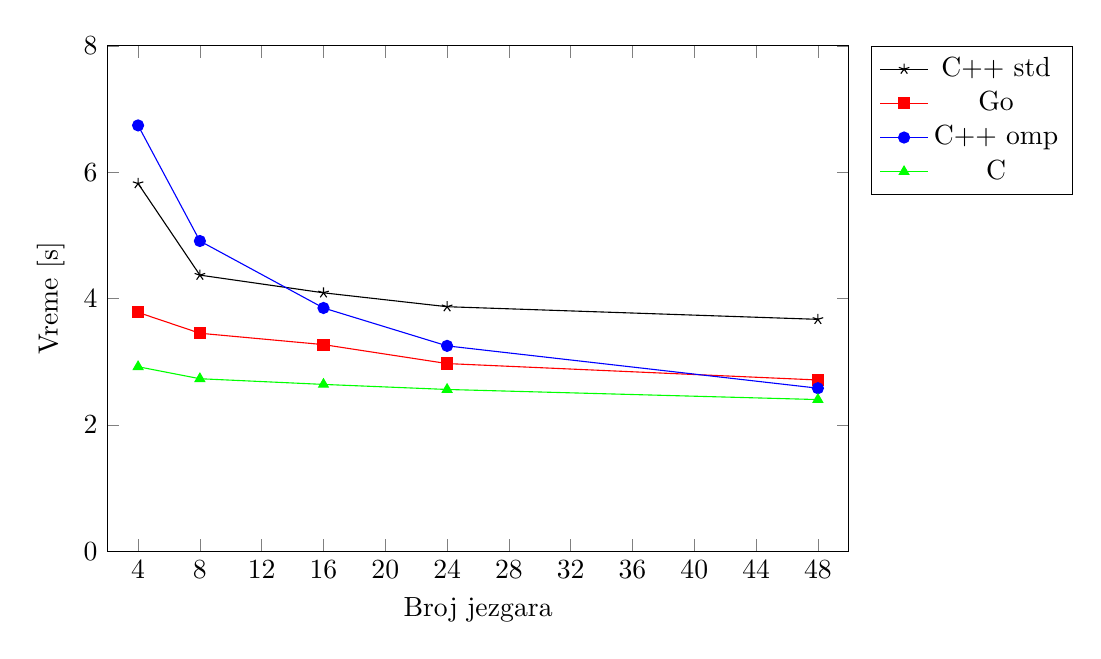
\begin{tikzpicture}
\begin{axis}[
    xlabel={Broj jezgara},
    ylabel={Vreme [s]},
    xmin=2, xmax=50,
    ymin=0, ymax=8,
    xtick={4,8,12,16,20,24,28,32,36,40,44,48},
    ytick={0,2,4,6,8},
    legend pos=outer north east,
    ymajorgrids=true,
    grid=none,
    width=11cm,
    height=8cm,
]

\addplot[black,mark=star] coordinates {(4,5.82)(8,4.37)(16,4.09 )(24,3.87)(48,3.67)};  
\addplot[red,mark=square* ]  coordinates {(4,3.78)(8,3.45)(16,3.27 )(24,2.97)(48,2.71)}; 
\addplot[blue,mark=*]  coordinates {(4,6.74)(8,4.91)(16,3.85 )(24,3.25 )(48,2.58)}; 
\addplot[green,mark=triangle*] coordinates {(4,2.92)(8,2.73)(16,2.64 )(24,2.56)(48,2.40)};

\legend{ C++ std, Go,C++ omp,C}
\end{axis}
\end{tikzpicture}

\caption{Grafik brzine izvršavanja različitih quicksort implementacija u zavisnosti od broja jezgara, testirano za niz od 10 miliona brojeva}
\label{fig:qs1}
\end{center}
\end{figure}

Maksimalna upotreba memorije za nizove različitih dužina je prikazana u tabeli \ref{tab:qs3}. Obe verzije u C++-u su podjednako efikasne i potrebno im je manje memorije u odnosu na druge implementacije. C je približno efikasan kao i C++ osim što i za nizove manjih dužina zahteva veliku količinu memorije. Go koristi dva puta više memorije nego ostale implementacije dok je Python-u potrebna višestruko veća količina memorije.
\\

\begin{table}
\begin{center}
\caption{Maksimalna upotreba memorije [MB] quicksort implementacija za različite dužine niza}
\begin{tabular}{||c||c|c|c||}
\hline
\diagbox[width=2.7cm, height=1cm]{Verzija}{\vspace*{-0.8cm}n [$10^{6}$]} &1 &10 &100 0 \\ \hline
C++ omp	& \textbf{6.3}	&\textbf{42.3}	&\textbf{393.1}	\\ 
C++ std	& 25.2		&55.0			&393.5		\\ 	
C 		& 58.1		&68.8			&408.5		\\ 
Go		& 13.4 		&87.5			&816.3		\\ 
Python thr	& 40.4		&396.3		& -			\\
Python pp	& 49.6		&411.8		& - 			\\ \hline
\end{tabular}
\label{tab:qs3}
\end{center}
\end{table}

Dužine implementacija, prikazane su u tabeli \ref{tab:qs4}.  Za implementaciju algoritma u C-u, potreban je najveći broj linija koda, dok je u Python-u potreban najmanji broj linija.

\begin{table}
\begin{center}
\caption{Dužine k\^{o}da quicksort implementacija}
\begin{tabular}{|c|c|c|c|c|c|c|}
\hline
		&  C 	& Go	& C++ std	& C++ omp	& Python pp & Python thr \\ \hline
Br. linija koda& 119	& 98	&84		&79		&55		&43	 \\ \hline
\end{tabular}
\label{tab:qs4}
\end{center}
\end{table}

\subsection{Rezime}

Za konkurentnu implementaciju \textit{quicksort} algoritma, Go se pokazao vremenski efikasan isto koliko C i C++ za nizove dužine do 10 miliona, dok mu je potrebno dva puta više vremena za nizove dužine od 100 miliona brojeva, ali prilkom sekvencijalnog izvršavanja ispostavio se kao najefikasniji. Što se tiče memorijskih zahteva, Go koristi dva puta više memorije nego C i C++, ali je i memorijski i vremenski višestruko efikasniji od Pythona. Dužina koda Go implementacije, uporediva je sa C-om i C++-om.

% Matrix==============================================================================

\section{Množenje matrica}
Za izradu implementacija, upotrebljen je standardni algoritam za \textit{množenje matrica}. Vrednost na poziciji \textit{ij} proizvoda matrica A i B, izračunava se kao: $$(AB)_{ij} = \sum_{k=1}^{n} A_{ik}B_{kj}$$ gde je \texttt{n} dužina matrice A. 

Algoritam je paralelizovan tako što svaka nit/gorutina računa po jedan red matrice, odnosno, jedan red prve matrice množi sa svim kolonama druge matrice. Za testiranje, korišćene su pseudoslučajno generisane kvadratne matrice različitih dimenzija. Kodovi svih implementacija, dostupni su na repozitorijumu\footnote{\url{https://github.com/MitrovicMilosh/Go-Concurrency/tree/master/matrix_multiplication}}.

\subsection{Go}
Restrikcija broja gorutina, ostvaruje se pomoću semafora na isti način kao što je urađeno u prethodnoj implementaciji u poglavlju \ref{qs:go}. U implementaciji prikazanoj u listingu\ref{lst:matrix}, može se primetiti da je neophodno gorutinama proselditi \texttt{i} kao argument anonimne funkcije kako bi svaka gorutina imala svoju kopiju. U suprotnom, u svakoj sledećoj iteraciji \texttt{for} petlje vrednost \texttt{i} bi bila ažurirana u svim gorutinama. Za razliku od prethodne implementacije gde se niz koji se sortira prenosi pomoću reference, ovde su matrice definisane kao globalne. Nije potrebno nikakvo zaključavanje jer se početne matrice koriste samo za čitanje, a kod rezultujuće matrice svaka gorutina popunjava samo svoj red. 

\begin{center}
\begin{lstlisting}[caption=Go implementacija konkurentne funkcije za množenje matrica,label={lst:matrix}, backgroundcolor=\color{background}]
func multiply(){
	wg := sync.WaitGroup{}
	wg.Add(n)

	for i := 0; i < n; i++ {
		select{
		case semaphore <- struct{}{}:
			go func(row int){
				multiply_row(row)
				<- semaphore
				wg.Done()
			}(i)
		default:
			multiply_row(i)
			wg.Done()
		}
	}

	wg.Wait()
}
\end{lstlisting}
\end{center}

\subsection{Ostale implementacije}
Implementacije u ostalim jezicima su realizovane na sličan način. Maksimalan broj niti koji se kreira u toku izvršavanja programa zadaje se unapred. Za C++ razmatrane su dve implementacije. Jedna implementacija je ostvarena pomoću \texttt{omp} biblioteke i koristi običan niz za reprezntaciju matrice, dok druga koristi strukturu vektor i standardnu biblioteku.


\subsection{Rezultati}

Grafik brzine izvršavanja u zavisnosti od veličine matrice, prikazan je na slici \ref{fig:matrix1}. Python se izvršava znatno sporije od ostalih implementacija tako da nije bilo mogućnosti testirati ga na ulazima iste veličine, a rezultati testiranja Python implementacije, prikazani su u posebnoj tabeli. Na osnovu grafika se zaključuje da je C implementacija najefikasnija, a zatim C++ verzija sa \texttt{omp} bibliotekom, dok C++ verzija sa standardnom bibliotekom radi najsporije. Za matrice manje veličine, Go radi podjednako efikasno kao i C++ \texttt{omp} verzija, ali za matricu veličine 1500, Go zahteva dva puta više vremena nego C++, što je približno četiri puta više nego C. 

\begin{figure}
\begin{center}

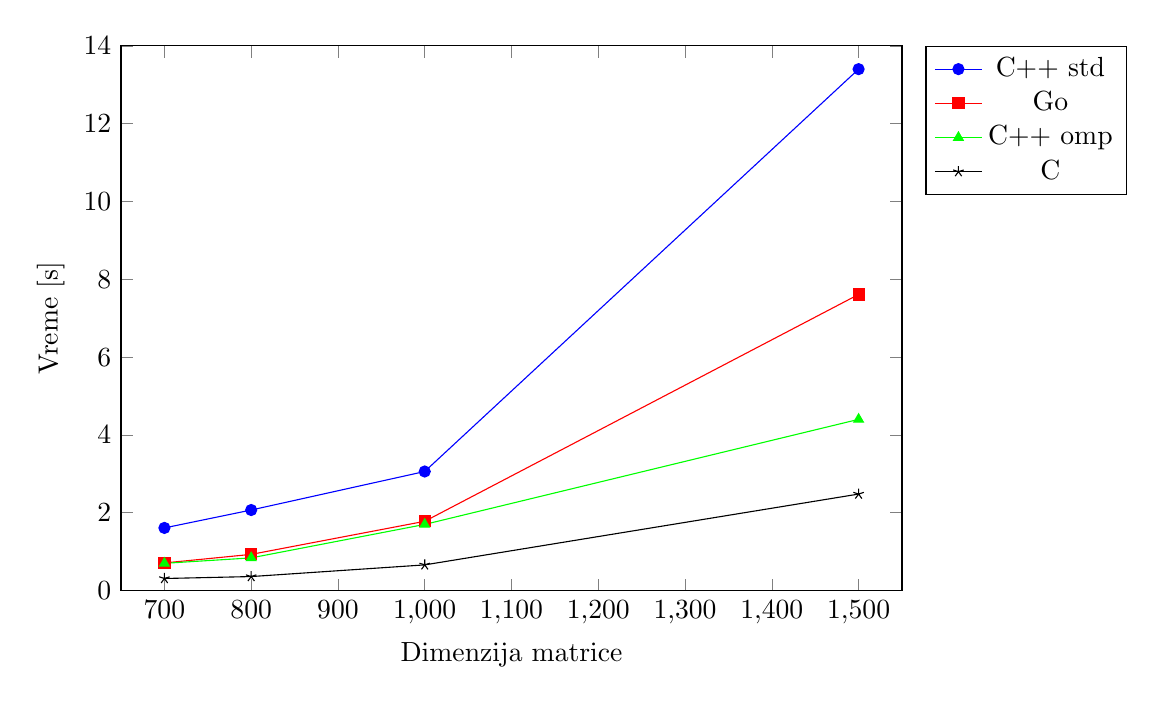
\begin{tikzpicture}
\begin{axis}[
    xlabel={Dimenzija matrice},
    ylabel={Vreme [s]},
    xmin=650, xmax=1550,
    ymin=0, ymax=14,
    xtick={700,800,900,1000,1100,1200,1300,1400,1500},
    ytick={0,2,4,6,8,10,12,14,16,18,20,22},
    legend pos=outer north east,
    ymajorgrids=true,
    grid=none,
    width=11.5cm,
    height=8.5cm,
]

\addplot[blue,mark=*] coordinates {(700,1.61 )(800,2.07 )(1000,3.06 )(1500,13.4 )}; 
\addplot[red,,mark=square*] coordinates {(700,0.71 )(800,0.93 )(1000,1.78)(1500,7.61 )}; 
\addplot[green,mark=triangle*] coordinates {(700,0.70 )(800,0.84 )(1000,1.70 )(1500,4.40 )}; 
\addplot[black,mark=star] coordinates {(700, 0.31)(800, 0.36)(1000, 0.66)(1500,2.48 )}; 
\legend{C++ std,Go, C++ omp,C}
\end{axis}
\end{tikzpicture}

\caption{Grafik brzine izvršavanja različitih implementacija množenja matrica u zavisnosti od veličine matrice, testirano na 48 jezgara}
\label{fig:matrix1}
\end{center}
\end{figure}


Prosečno vreme izvršavanja sa različitim brojem niti za matricu veličine 1000, prikazano je u tabeli \ref{tab:matrix5}. Najbolje vreme se postiže sa 100 niti/gorutina za Go i C++ \texttt{omp} verziju i sa 1000 niti za C i C++ verziju sa standardnom bibliotekom. Kod ostalih testiranja, korišćen je onaj broj niti/gorutina za koji implementacija pokazuje najbolje rezultate. 
\\

\begin{table}
\begin{center}
\caption{Prosečno vreme izvršavanja [s] implementacija množenja matrica sa različitim brojem niti, testirano sa 48 jezgara za matrice veličine 1000}
\begin{tabular}{||c||c c c c||}
\hline
Br. niti		&10&30 &100 &1000\\ \hline
Go		&6.39	&3.01&\textbf{1.78}&1.82	 \\ \hline
C		&2.74	&1.39&0.92&\textbf{0.81} \\ \hline
C++ omp	&3.03	&1.95&\textbf{1.70}&1.97 \\ \hline
C++ std	&15.31&8.71&3.21&\textbf{3.06} \\ \hline
\end{tabular}
\label{tab:matrix5}
\end{center}
\end{table}

Rezultati testiranja implementacija na različitom broju jezgara, prikazani su na slici \ref{fig:matrix3}. Na grafiku se može videti velika razlika u brzini između sekvencijalnog (na jednom jezgru) i konkurentnog izvršavanja. Brzina izvršavanja raste do 16 i 24 jezgara, dok povećanje na 48 jezgara, ne donosi značajno ubrzanje. 
\\

\begin{figure}
\begin{center}

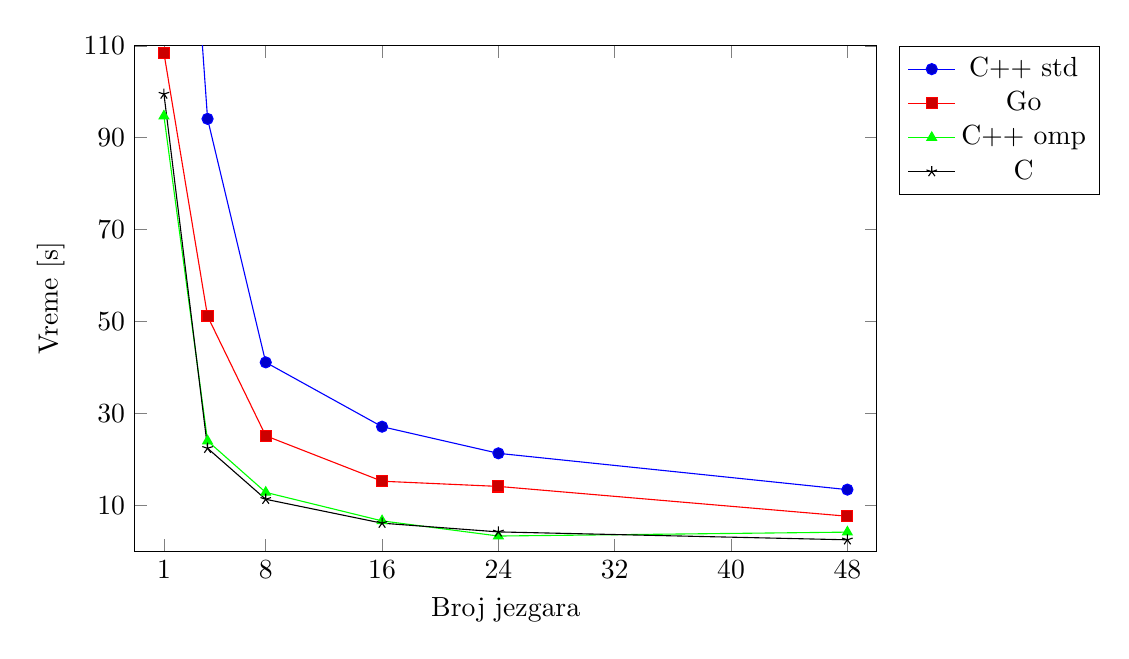
\begin{tikzpicture}
\begin{axis}[
    xlabel={Broj jezgara},
    ylabel={Vreme [s]},
    xmin=-1, xmax=50,
    ymin=0, ymax=110,
    xtick={1,8,16,24,32,40,48},
    ytick={10,30,50,70,90,110},
    legend pos=outer north east,
    ymajorgrids=true,
    grid=none,
    width=11cm,
    height=8cm,
]
\addplot coordinates {(1, 229)(4,94.1)(8,41.1)(16,27.1 )(24,21.3 )(48,13.4)}; 
\addplot coordinates {(1,108.4 )(4,51.14)(8,25.12)(16,15.23 )(24,14.1 )(48,7.61)}; 
\addplot[green,mark=triangle*]  coordinates {(1,94.7 )(4,24)(8,12.8)(16,6.6 )(24,3.3 )(48,4.15)}; 
\addplot coordinates {(1,99.5 )(4,22.4)(8,11.3)(16,6.1 )(24,4.2 )(48,2.48)}; 


\legend{C++ std, Go, C++ omp, C}
\end{axis}
\end{tikzpicture}

\caption{Grafik brzine izvršavanja različitih implementacija množenja matrica u zavisnosti od broja jezgara za matricu veličine 1500}
\label{fig:matrix3}
\end{center}
\end{figure}

Rezultati python implementacije, prikazani su u tabeli \ref{tab:matrix1}. Python se izvršava višestruko sporije i potrebno mu je više od 90 sekundi za matricu veličine 500, dok je ostalim implementacijama potrebno manje od jedne sekunde. Konkurentno izvršavanje je ponovo sporije od sekvencijalnog zbog već pomenutog problema sa GIL-om u poglavlju \ref{gil}.
\\

\begin{table}
\begin{center}
\caption{Prosečno vreme izvršavanja i maksimalna upotreba memorije Python implementacije množenja matrica za različito n}
\begin{tabular}{||c||c|c|c||}
\hline
n & Konkurentno [s]& Sekvencijalno [s] & Memorija [MB] \\ \hline
100	&0.78	&0.32&7.5\\
300	&21.11&7.59&10.0\\
500	&97.73&38.27&17.4\\
\hline
\end{tabular}
\label{tab:matrix1}
\end{center}
\end{table}

Grafik maksimalne upotrebe memorije u zavisnosti od dimenzije matrica, prikazan je na slici \ref{fig:matrix2}. Memorijska efikasnost implementacija se poklapa sa vremenskom. C i C++ \texttt{omp} vezija su najefikasnije dok Go koristi dva puta više memorije. C++ verzija sa standardnom bibliotekom zahteva najveću količinu memorije. 
\\

\begin{figure}
\begin{center}

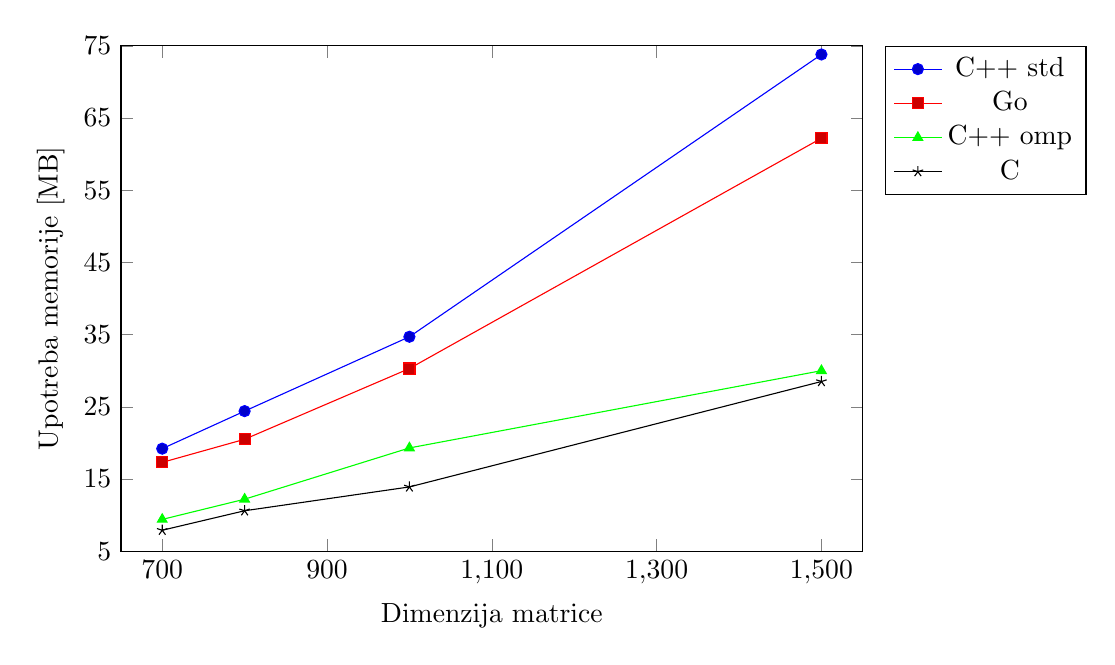
\begin{tikzpicture}
\begin{axis}[
    xlabel={Dimenzija matrice},
    ylabel={Upotreba memorije [MB]},
    xmin=650, xmax=1550,
    ymin=5, ymax=75,
    xtick={700,900,1100,1300,1500},
    ytick={5,15,25,35,45,55,65,75},
    legend pos=outer north east,
    ymajorgrids=true,
    grid=none,
    width=11cm,
    height=8cm,
]
\addplot coordinates {(700, 19.2)(800, 24.4)(1000, 34.7)(1500,73.8 )}; 
\addplot coordinates {(700,17.3 )(800,20.5 )(1000,30.3 )(1500,62.2)}; 
\addplot[green,mark=triangle*] coordinates {(700,9.4 )(800,12.2 )(1000,19.3 )(1500,30 )}; 
\addplot[black,mark=star] coordinates {(700,7.9 )(800,10.6 )(1000,13.9)(1500,28.5)}; 
\legend{ C++ std,Go, C++ omp,C}
\end{axis}
\end{tikzpicture}

\caption{Grafik maksimalne upotrebe memorije različitih implementacija množenja matrica u zavisnosti od dimenzije matrica}
\label{fig:matrix2}
\end{center}
\end{figure}


Broj linija koda svih  implementacija, prikazan je u tabeli \ref{tab:matrix2}. Python ima najkraću implementaciju sa samo 28 linija koda. Najduža implementacija je C++ verzija sa standardnom bibliotekom usled razdvajanja na klase i nekoliko fajlova radi jednostavnijeg korišćenja.  

\begin{table}
\begin{center}
\caption{Dužine k\^{o}da implementacija množenja matrica}
\begin{tabular}{|c|c|c|c|c|c|}
\hline
		& C++ std	&  Go 	& C	& C++ omp	& Python	\\ \hline
Br. linija koda&170		& 75	& 70	&50		&28		\\ \hline
\end{tabular}
\label{tab:matrix2}
\end{center}
\end{table}

\subsection{Rezime}

Za konkurentnu implementaciju algoritma \textit{množenja matrica}, Go se pokazao vremenski efikasan koliko C i C++ za ulaze manjih dimenzija, dok za velike ulaze zahteva dva puta više vremena. Takođe, potrebna mu je dva puta veća količina memorije ali je neuporedivo vremenski i memorijski efikasniji od Python-a. Potreban je približno isti broj linija k\^{o}da za implementaciju algoritma koliko i u C-u.

% Prime==============================================================================

\section{Eratostenovo sito} \label{erathost}
Eratostenovo sito je algoritam za određivanje prostih brojeva manjih od n. Ideja algoritma je da se eliminišu svi brojevi koji nisu prosti između 2 i \texttt{n}. Na početku se pretpostavlja da su svi brojevi prosti, odnosno definiše se niz od \texttt{n} bulovskih vrednosti postavljenih na \texttt{true}. Polazi se od prvog prostog broja što je 2, tako što se eliminiše svaki drugi broj počevši od $2^{2}$, a zatim, prelazi se na sledeći prost broj i postupak se ponavlja. Uopšteno, za \texttt{i}-ti prost broj eliminiše se svaki i-ti broj počevši od  $\texttt{i}^{2}$. Postupak je dovoljno ponoviti za proste brojeve koji su manji od $\sqrt{\texttt{n}}$. Pseudokod algoritma je prikazan na slici \ref{fig:prime_pseudo}.

\begin{figure}
\begin{center}

\begin{Verbatim}[fontsize=\small]
for i:=2 to n do
    A[i]:=true

ErathostenesSieve(n):
    for i:=2 to floor(sqrt(n)) do 
         if A[i] = true:
             j := i * i
             while j < n do
                 A[j] := false 
                 j := j + i
\end{Verbatim}

\caption{Pseudokod algoritma Eratostenovo sito}
\label{fig:prime_pseudo}
\end{center}
\end{figure}

Paralelizacija algoritma se postiže deljenjem opsega od 2 do \texttt{n} na jednake delove. Svaka nit/gorutina dobija svoj deo opsega u okviru kojeg eliminiše brojeve koji nisu prosti. Za svaki prost broj je prvo potrebno odrediti njegov prvi umnožak unutar opsega. Iako svaka nit/gorutina ima svoj opseg, ona mora da pristupa članovima niza drugih niti/gorutina jer su joj potrebni svi prosti brojevi manji od $\sqrt{\texttt{n}}$. To kao posledicu dovodi do mogućnosti da se u nekim slučajevima bespotrebno eliminišu umnošci brojeva koji nisu prosti ukoliko ih druga nit/gorutina još uvek nije eliminisala. Problem je rešen tako što se proverava dodatni uslov prilikom eliminacije: da li je neka druga nit/gorutina u međuvremenu označila da taj broj nije prost. Kodovi svih implementacija, dostupni su na repozitorijumu\footnote{\url{https://github.com/MitrovicMilosh/Go-Concurrency/tree/master/prime_sieve}}.

\begin{center}
\begin{lstlisting}[caption=Go implementacija konkurentne funkcije za određivanje prostih brojeva manjih od n,label={lst:prime1},backgroundcolor=\color{background}]
func Prime(list *[]bool, n int, is_concurrent bool){
	sqrt := int(math.Sqrt(float64(n)))
	first := 0
	step := int(n/ num_goroutines)
	last := step
	wg := sync.WaitGroup{}
	wg.Add(num_goroutines)

	for i:=0; i < num_goroutines-1; i++{
		go mark_prime(list,first,last,sqrt,&wg,true)
		first = last + 1
		last += step
	}

	mark_prime(list,first,n-1,sqrt,&wg)
	wg.Wait()
}
\end{lstlisting}
\end{center}

\subsection{Go}

Koristi se globalni niz od \texttt{n} bulovskih promenljivih postavljenih na podrzumevanu vrednost \texttt{false} umesto na \texttt{true} radi jednostavnosti.  Funkcija koja kreira gorutine, prikazana je u listingu \ref{lst:prime1}. Za svaki broj koji je trenutno označen kao prost, najpre je potrebno je odrediti njegov prvi umnožak, a zatim, označiti sve njegove umnoške unutar opsega, što je i prikazano u listingu \ref{lst:prime2}. Kao što je već pomenuto, ako svaka gorutina ima svoj opseg, ona mora da pristupa i članovima niza drugih gorutina jer su joj potrebni svi prosti brojevi manji od $\sqrt{\texttt{n}}$. To kao posledicu dovodi do pojave trke za resursima, međutim, u ovom slučaju je to dopustivo i nisu potrebni muteksi, upravo zato što se proverava dodatni uslov da li je pročitana vrednost u međuvremenu bila menjana. Ako se detektor trke za resurse pozove, dobija se izveštaj koji upozorava da je ona prisutna. Primer izveštaja se može videti u poglavlju \ref{datarace}na slici \ref{fig:datarace}. 

\begin{center}
\begin{lstlisting}[caption=Go implementacija konkurentne funkcije za označavanje prostih brojeva,label={lst:prime2}, backgroundcolor=\color{background}]
func mark_prime(list *[]bool,first,last,sqrt int,wg *sync.WaitGroup){
	for i:=2;  i<= sqrt && i*i<= last; i++{
		if !(*list)[i] {
			var j int
			if i*i < first {
				if (first - i*i)%i == 0 {
					j = i*i + ((first-i*i)/i)*i
				}else {
					j = i*i + ((first-i*i)/i + 1)*i
				}
			}else {
				j = i*i
			}
		
			for ; j <= last && !(*list)[i]; j+=i {
				(*list)[j] = true
			}
		}
	}
	wg.Done()
}
\end{lstlisting}
\end{center}

\subsection{Ostale implementacije}
Implementacije u ostalim jezicima su realizovane na isti načini. Za C++ je razmatrana samo jedna implementacija koja koristi \texttt{omp} biblioteku.

\subsection{Rezultati}

Prosečno vreme konkurentnog i sekvencijalnog izvršavanja implementacija, predstavljeno je grafikom na slici \ref{fig:prime1}. Python nije mogao da bude uključen na ovom grafiku usled znatno sporijeg izvršavanja, a rezultati Python implementacije, prikazani su u posebnoj tabeli. Go implementacija se pokazala kao najefikasnija. C++ implementacija je približno efikasna koliko je i Go, i obe rade ispod jedne sekunde za najveći ulaz. C implementacija je znatno sporija i njeno izvršavanje se meri u sekundama. U odnosu na sekvencijano izvršavanje, Go ima najveće ubrzanje. Pri konkurentnom izvršavanju, veličina ulaza nema značajan uticaj i nema velike razlike u brzini kada \texttt{n} iznosi 500 miliona ili 1 milijardu. 
\\

\pgfplotsset{ every non boxed x axis/.style={} }

\begin{figure}
\begin{center}

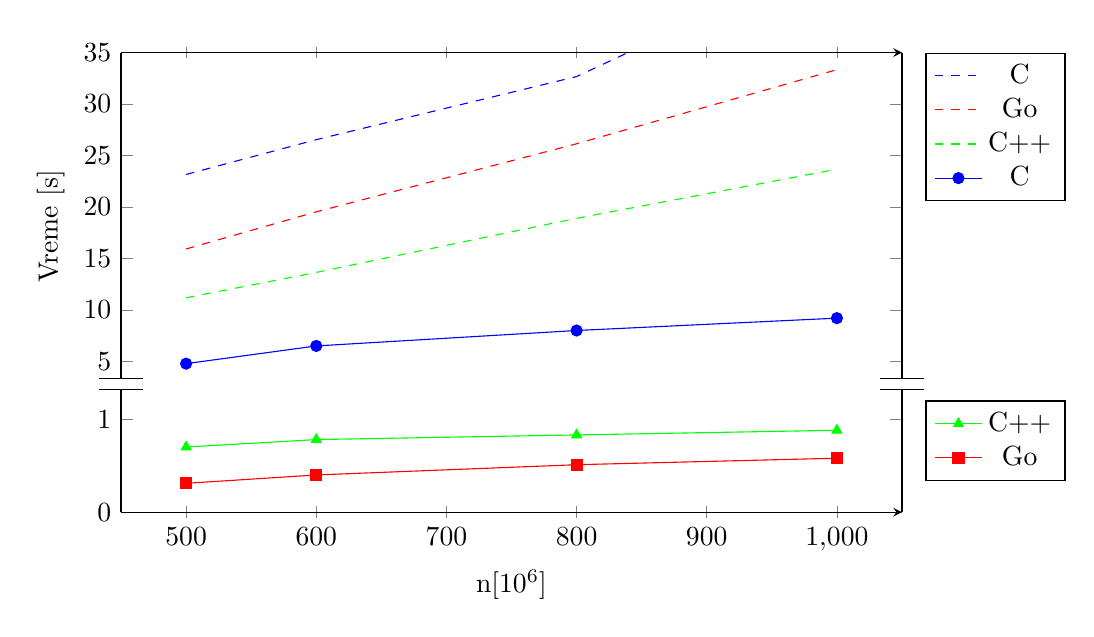
\begin{tikzpicture}
\begin{groupplot}[
    group style={
        group name=my fancy plots,
        group size=1 by 2,
        xticklabels at=edge bottom,
        vertical sep=0cm
    },
    xlabel={n[$10^{6}$]},
    ylabel={Vreme [s]},
    xmin=450, xmax=1050,
    xtick={500,600,700,800,900,1000},
    legend pos=outer north east,
    ymajorgrids=true,
    grid=none,
    width=11.5cm,
]


\nextgroupplot[ymin=1.2,ymax=35,
               ytick={5,10,15,20,25,30,35},
               axis x line=top, 
               axis y discontinuity=parallel,
               height=6.0cm,
	    xlabel={}]

\addplot[blue, dashed] coordinates {(500,23.16 )(600,26.54)(800,32.67 )(1000, 44.47)};
\addplot[red, dashed] coordinates {(500, 15.92 )(600,19.53)(800,26.14 )(1000, 33.34)};   
\addplot[green, dashed] coordinates {(500, 11.18 )(600,13.64)(800,18.9 )(1000, 23.67)};
\addplot[blue,mark=*] coordinates {(500,4.78 )(600,6.5)(800,8 )(1000, 9.2)}; 
\legend{C,Go,C++,C}


\nextgroupplot[ymin=0,ymax=1.2,
               ytick={0,1},
               axis x line=bottom,
               height=3.0cm, ylabel={}]


\addplot[green,mark=triangle*] coordinates {(500, 0.7)(600,0.78)(800,0.83 )(1000,0.88 )}; 
\addplot[red,mark=square*] coordinates {(500,0.31 )(600,0.4)(800,0.51 )(1000,0.58 )}; 
\legend{C++,Go}

\end{groupplot}
\end{tikzpicture}
\caption{Grafik brzine izvršavanja različitih implementacija Eratostenovog sita za različito n, testirano na 48 jezgara; isprekidanom linjom je prikazano sekvencijalno izvršavanje dok je konkurentno prikazano punom linijom}
\label{fig:prime1}

\end{center}
\end{figure}

U tabeli \ref{tab:prime5}, prikazano je vreme izvršavanja sa različitim brojem niti/gorutina kada je n = 500 miliona. Sve tri implementacije postižu najbolje performanse sa 1000 niti/gorutina što je iskorišćeno prilikom svih ostalih testiranja.

\begin{table}
\begin{center}
\caption{Prosečno vreme izvršavanja [s] implementacija Eratostenovog sita sa različitim brojem niti, testirano sa 48 jezgara za n = 500 miliona}
\begin{tabular}{||c||c c c c||}
\hline
Br. niti		&10 &100 &1000 &10000\\ \hline
Go	&2.14	&0.40	&\textbf{0.31}&0.49\\ \hline
C	&6.17	&4.81	&\textbf{4.74}&7.85\\ \hline
C++  &4.53	&2.84	&\textbf{0.73}&0.76\\ \hline
\end{tabular}
\label{tab:prime5}
\end{center}
\end{table}


Grafik brzine izvršavanja implementacija u zavisnosti od broja jezgara, prikazan je na slici \ref{fig:prime3}. Kod svih implementacija postoji ubrzanje sa povećanjem broja jezgara, ali ne postoji značajna razlika u brzini prilikom izvršavanja sa 24 i 48 jezgara.
\\

\begin{figure}
\begin{center}

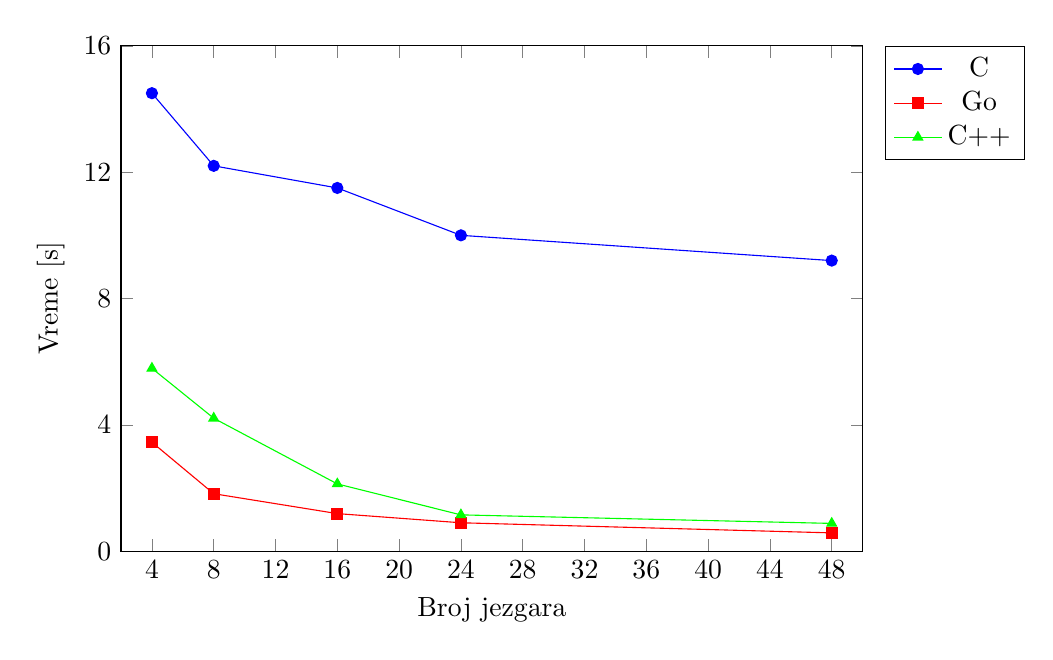
\begin{tikzpicture}
\begin{axis}[
    xlabel={Broj jezgara},
    ylabel={Vreme [s]},
    xmin=2, xmax=50,
    ymin=0, ymax=16,
    xtick={4,8,12,16,20,24,28,32,36,40,44,48},
    ytick={0,4,8,12,16},
    legend pos=outer north east,
    ymajorgrids=true,
    grid=none,
    width=11cm,
    height=8cm,
]
\addplot[blue,mark=*] coordinates {(4,14.5)(8,12.2)(16,11.5)(24,10.0 )(48,9.20)}; 
\addplot[red,mark=square* ]   coordinates {(4,3.45)(8,1.82)(16,1.19 )(24,0.90 )(48,0.58)}; 
\addplot[green,mark=triangle*] coordinates {(4,5.79)(8,4.21)(16,2.13 )(24,1.15)(48,0.88)}; 
\legend{C, Go, C++}
\end{axis}
\end{tikzpicture}

\caption{Grafik brzine izvršavanja različitih implementacija Eratostenovog sita u zavisnosti od broja jezgara}
\label{fig:prime3}
\end{center}
\end{figure}

Python je testiran za deset puta manju vrednost \texttt{n} u odnosu na ostale implementacije i rezultati testiranja su prikazani u tabeli \ref{tab:prime1}. Prilikom izvršavanja algoritma, Python-u je potrebno više od jednog minuta, dok Go za deset puta veću vrednost radi ispod jedne sekunde. Upotreba memorije je četiri puta veća nego kod ostalih implementacija i potrebno je više vremena pri konkurentnom izvršavanju nego pri sekvencijalnom usled već pomenutog problema sa GIL-om u odeljku \ref{gil}.
\\

\begin{table}
\begin{center}
\caption{Prosečno vreme izvršavanja i maksimalna upotreba memorije Python implementacije Eratostenovog sita za različito n}
\begin{tabular}{||c||c|c|c||}
\hline
n[$10^{6}$] & Konkurentno [s]& Sekvencijalno [s] & Memorija [MB] \\ \hline
1	&0.57	&0.32&13.5\\
10	&9.92&3.53&51.0\\
30	&32.18&12.04&129.9\\
50	&52.76&19.42&201.2\\
100	&113.80&57.58&397.1\\
\hline
\end{tabular}
\label{tab:prime1}
\end{center}
\end{table}

Maksimalna upotreba memorije u zavisnosti od \texttt{n}, prikazana je na slici \ref{fig:prime2}. Sve tri implementacije imaju slične memorijske zahteve. Na grafiku se vidi približno linearna zavisnost y=x, što znači da je potrebna količina memorije direktno proporcijalna vrednosti \texttt{n}.
\\

\begin{figure}
\begin{center}

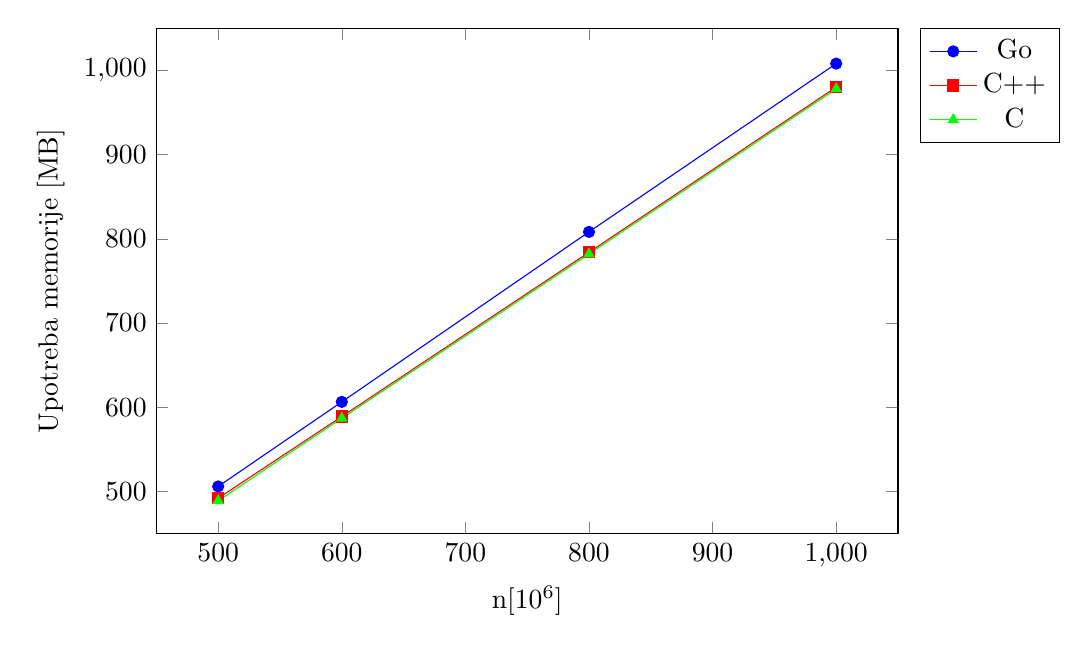
\begin{tikzpicture}
\begin{axis}[
    xlabel={n[$10^{6}$]},
    ylabel={Upotreba memorije [MB]},
    xmin=450, xmax=1050,
    ymin=450, ymax=1050,
    xtick={500,600,700,800,900,1000},
    ytick={500,600,700,800,900,1000},
    legend pos=outer north east,
    ymajorgrids=true,
    grid=none,
    width=11cm,
    height=8cm,
]
\addplot[blue,mark=*] coordinates {(500,506 )(600,606.4)(800,808.2)(1000,1008 )}; 
\addplot[red,mark=square* ]coordinates {(500,492)(600,589)(800,784)(1000,980 )}; 
\addplot[green,mark=triangle*] coordinates {(500,489 )(600,587)(800,782 )(1000, 978)}; 
\legend{Go, C++,C}
\end{axis}
\end{tikzpicture}

\caption{Grafik maksimalne upotrebe memorije različitih implementacija Eratostenovog sita za različito n}
\label{fig:prime2}
\end{center}
\end{figure}

Dužine implementacija su prikazane u tabeli \ref{tab:prime2}. Najkraća implementacija algoritma je u Python-u, dok je u C-u najduža. Go se ponovo nalazi između C-a i C++-a po broju linija koda.

\begin{table}
\begin{center}
\caption{Dužine k\^{o}da implementacija Eratostenovog sita}
\begin{tabular}{|c|c|c|c|c|}
\hline
		&  C  		&Go 	& C++ & Python 	 \\ \hline
Br. linija koda& 89		& 78	&61	&42		 \\ \hline
\end{tabular}
\label{tab:prime2}
\end{center}
\end{table}


\subsection{Rezime}

Za implementaciju algoritma \textit{Eratostenovo sito}, Go implementacija se ispostavila kao vremenski najefikasnija sa značajnim ubrzanjem u odnosu na sekvencijalno izvršavanje. Upotreba memorije je približno ista kolika je kod C-a i C++-a, kao i dužina koda implementacije.

%Aplikacija================================================================

\chapter{Primer upotrebe programskog jezika Go}

Kao primer upotrebe programskog jezika Go, razvijena je serverska aplikacija\ koja demonstrira korišćenje konkurentnosti kao i drugih aspekata jezika. U ovoj glavi, predstavljena je struktura aplikacije i opisani su pojedinačni delovi koji ilustruju različite karakteristike programskog jezika. 

\section{Serverska aplikacija}

Razvijena serverska aplikacija se bavi primenom različitih filtera na slikama. Omogućava primenu postojećih predefinisanih filtera kao i kreiranje sopstvenog, kombinovanjem različitih ponuđenih filtera i unošenjem željenih vrednosti za pojedine karakteristike. Slika koje se obrađuje se može upload-ovati sa računara ili se može proslediti njen URL. Svi filteri se primenjuju paralelno nakon čega se mogu videti pojedinačni rezultati obrade koji su dostupni za preuzimanje. Kompletan kod aplikacije je dostupan na repozitorijumu\footnote{\url{https://github.com/MitrovicMilosh/Go-Concurrency/blob/master/server/server.go}}. Za razvoj, korišćena je Go 1.8 verzija programskog jezika. Grafički interfejs aplikacije je prikazan na slici \ref{fig:interface}.

\begin{figure}
\begin{center}
\includegraphics[scale=1.4]{interface.png}
\end{center}
\caption{Grafički interfejs početne stranice i stranice za prikaz rezultata serverske aplikacije za primenu filtera}
\label{fig:interface}
\end{figure}

\subsection{Struktura aplikacije}
Struktura aplikacije predtsavljena je dijagramom na slici \ref{fig:diag}. Server, na osnovu zahteva koji dobija od korisnika, poziva odgovarajuću hendler funkciju. Definisane su dve hendler funkcije: \texttt{DefuaultHandle}, koja ima zadatak da generiše početnu HTML stranicu, i \texttt{ImageHandler}, koja se bavi preuzimanjem i procesiranjem fajla, primenom filtera na slici i generisanjem HTML stranice za prikaz rezultata. 
 
\begin{figure}
\begin{center}
\includegraphics[scale=0.45]{dijagram.png}
\end{center}
\caption{Dijagram koji prikazuje strukturu aplikacije}
\label{fig:diag}
\end{figure}

\subsection{Kreiranje servera i procesiranje zahteva}

Za kreiranje servera je korišćen \texttt{net/http} paket koji obezbeđuje skup funkcija za jednostavnu implementaciju i upravljanje serverom. Primer jednog jednostavnog servera je prikazan na listingu \ref{lst:server1}. 

\begin{center}
\begin{lstlisting}[caption=Primer jednostavnog servera,label={lst:server1},   backgroundcolor=\color{background}]
package main
import ("net/http"; "fmt")

func hello(w http.ResponseWriter, r *http.Request) {
	fmt.Fprintln(w,"Hello!")
}
func main() {
	http.HandleFunc("/", hello)
	http.ListenAndServe(":12345", nil)
}
\end{lstlisting}
\end{center}


Funkcija \texttt{HandleFunc} se koristi za registrovanje hendler funkcija za određeni šablon. Kao parametre, hendler funkcija ima \texttt{ResponseWriter} koji se koristi za konstrukciju HTTP odgovora i \texttt{Request} koji sadrži sve podatke HTTP zahteva. Funkcija \texttt{ListenAndServe} osluškuje na zadatoj adresi (prvi parametar) TCP mreže i poziva \texttt{Serve} funkciju kojoj prosleđuje \texttt{Handler} (drugi parametar). U pozadini, funkcija \texttt{Serve} kreira novu gorutinu za svaku HTTP konekciju i poziva \texttt{Handler}. Ukoliko je \texttt{Handler} \texttt{nil}, koristi se \texttt{DefaultServeMux} multiplekser koji uparuje URL zahteve sa registrovanim šablonima i poziva odgovarajuću hendler funkciju \cite{http}.

Server se može implementirati u Go-u  koristeći samo dva paketa i manje od deset linija koda što je karakateristično za dinamički tipizirane, interpretirane jezike kao što su Python, PHP, Ruby i drugi. U C/C++ -u, koji su statički tipizirani jezici koji se kompiliraju, kao što je i Go, je potrebno devet bibiloteka i više od pedeset linija koda \cite{server}.

Deo koda koji se odnosi na kreiranje servera u aplikaciji, nalazi se u \texttt{main} funkciji koja je prikazana u listingu \ref{lst:main}. \texttt{HandleFunc} funkcijom, registrovane su dve hendler funkcije: \texttt{DefaultHandler} koja se poziva kada se pristupa početnoj strani i \texttt{ImageHandler} koja se poziva prilikom obrade slike i prikazivanja rezultata. \texttt{Handle} funkcija se koristi za registrovanje \texttt{Handler}-a za fajl sistem i šablona koji se odnosi na zahteve resursa.  U \texttt{ListenAndServe} funkciji je postavljeno da se osluškuje na http portu zadate adrese servera koja je u ovom slučaju postavljena na \texttt{localhost}.

\begin{center}
\begin{lstlisting}[caption={Funkcija \texttt{main}, kreiranje servera},label={lst:main},  backgroundcolor=\color{background},belowskip=-0.7 \baselineskip ]
func main() {
	fmt.Println("Starting server...")
	rand.Seed(time.Now().UTC().UnixNano())
	http.HandleFunc("/", DefaultHandler)
	http.HandleFunc("/results", ImageHandler)
	http.Handle("/data/", http.HandlerFunc(file_server))
	http.ListenAndServe(address + ":http", nil)
}
\end{lstlisting}
\end{center}

\label{fileserver}Hendler za fajl sistem je prikazan u listingu \ref{lst:fileserver}. U ovoj funkciji definišu se restrikcije nad URL zahtevima za resurse i definiše se \texttt{root} direktorijum svih resursa. URL se deli na segmente funkcijom split i zatim se ispituje poslednji segment. Ukoliko je poslednji segment prazan odnosno ako se URL završava znakom \texttt{/}, to znači da u zahtevu nije tražen određeni fajl već je u pitanju samo deo putanje. \texttt{DefaultServeMux} funkcioniše tako što dodaje znak \texttt{/} na kraju svakog URL zahteva koji postoji u podstablu root direktorijuma, što znači da ako korisnik unese putanju do nekog direktorijuma, poslednji deo URL zahteva će biti prazan \cite{http}. U tom slučaju korisniku će biti onemogućen pristup direktorijumu i neće moći da pročita njegov sadržaj.

\begin{center}
\begin{lstlisting}[caption=Hendler za fajl sistem,label={lst:fileserver},  backgroundcolor=\color{background}]
func file_server(w http.ResponseWriter, r *http.Request) {
	parts := strings.Split(r.URL.Path, "/")
	last := parts[len(parts)-1]
	if last == "" {
		http.NotFound(w, r)
		return
	}
	fileServer := http.StripPrefix("/data/", 
				http.FileServer(http.Dir("data"))).ServeHTTP(w, r)
}
\end{lstlisting}
\end{center}

\subsection{Generisanje HTML stranice}

Paket \texttt{htmp/template} koristi se za generisanje HTML izlaza sa datim parametrima koji ima zaštitu protiv umetanja koda. Paket nudi veliki broj različitih escape funkcija koje kodiraju specijalne karaktere, ali u ovoj aplikaciji nije bilo potrebe za njihovom upotrebom. 

U \texttt{DefaultHandler} funkciji, parsira se i izvršava šablon koji se prikazuje kada se pristupi početnoj strani. Deo funkcije koji se odnosi na izvršavanje šablona je prikazan u listingu \ref{lst:tmpl}. Ovde, kao i na drugim mestima, moguće greške će biti ignorisane jer se podrazumeva da su parametri funkcije ispravni i da neće doći do greške. Fiksni parametri su provereni tokom faze razvijanja i debagovanja aplikacije, dok parametri koji zavise od unosa korisnika, prethodno prolaze kroz odgovarajuće provere. Funkcija \texttt{ExecuteTemplate} kao argumente prima \texttt{ResponseWriter}, naziv šablona koji se izvršava i podatke koji se koriste za njegovo popunjavanje. Prosleđena promenljiva \texttt{data} je definisana struktura koja sadrži podatke o filterima u obliku mapa.

\begin{center}
\begin{lstlisting}[caption=Izvršavanje HTML šablona,label={lst:tmpl},  backgroundcolor=\color{background}]
func DefaultHandler(w http.ResponseWriter, r *http.Request) {
	...
	tmpl, _ := template.ParseFiles("index.html")
	tmpl.ExecuteTemplate(w, "index", data)
}
\end{lstlisting}
\end{center}

U šablonu se sve instrukcije, podaci i kontrole toka navode između dvostrukih vitičastih zagrada. Primer šablona je prikazan u listingu \ref{lst:tmpl2}. Na početku svakog šablona pomoću \texttt{define} se definiše naziv, a kraj šablona je potrebno naznačiti sa \texttt{end}. Omogućeno je iteriranje nad prosleđenim podacima, \texttt{if-else} naredbe i izvršavanje šablona unutar šablona. U ovom slučaju, iterira se nad mapom \texttt{Filters} koja sadrži nazive filtera i putanje do njihovih slika. Prosleđeni podaci počinju znakom \texttt{.} , dok promenljive počinju znakom \texttt{\$} \cite{template}.

\begin{center}
\begin{lstlisting}[caption=Izvršavanje HTML šablona,label={lst:tmpl2},  backgroundcolor=\color{background}]
{{define "index"}}
<html lang="en">
	<head>
		<meta charset="UTF-8">
		<title>Image Filters</title>
	</head>
	<body>
		...
		{{range $name, $image := .Filters}}
		<div class="gallery">
			<img src="{{$image}}" >
			<div class="desc">{{$name}}</div>
		</div>
		{{end}}
		...
	</body>
</html>
{{end}}
\end{lstlisting}
\end{center}

\subsection{Preuzimanje i procesiranje fajla}

Funkcija \texttt{ImageHandler} se poziva kada korisnik klikne na dugme filter i bavi se preuzimanjem fajla, proverom zadovoljenosti svih uslova i primenom filtera. Struktura funkcije je prikazana u listingu \ref{lst:imghand}. Unutar funkcije, nalazi se jedna \texttt{select} naredba. Za kontrolu maksimalnog broja konekcija koji server može da opsluži, koristi se semafor. Ukoliko ima slobodnih mesta, izvršiće se glavni deo funkcije. Ukoliko nema slobodnih mesta, nakon isteka dozvoljenog vremena čekanja \texttt{timeout}, korisniku se ispisuje poruka da je server trenutno zauzet. 
 
Deo funkcije koji se odnosi na otvaranje i proveru fajla, prikazan je u listingu \ref{lst:open}. U funkciji se koriste dve korisnički definisane strukture: \texttt{file\_info}, koja sadrži neophodne informacije o fajlu (naziv, veličina, referenca na otvoreni fajl, čitač fajla), i \texttt{processor}, tip nad kojim su definisani metodi koji koriste \texttt{ResponseWriter} i \texttt{Request} kako se ne bi prosleđivali pojedinačno svakoj funkciji koja ih koristi. Ovi metodi tokom svog rada proveravaju da li je došlo do neke greške pa kao rezultat vraćaju \texttt{bool} promenljivu kako bi funkcija \texttt{ImageHandler} prestala sa daljim radom. Generalno, validaciju fajla je prirodnije raditi na strani klijenta u javascript-u kako ne bi opterećivali server lošim zahtevima, ali u ovom slučaju demonstrirano je kako se validacija izvršava u Go-u.

\begin{center}
\begin{lstlisting}[caption=Struktura ImageHandler funkcije,label={lst:imghand},  backgroundcolor=\color{background}]
func ImageHandler(w http.ResponseWriter, r *http.Request) {
	select {
	case semaphore <- struct{}{}:
		...
	case <- time.After(timeout):
		ErrorHandler(w,"Server too busy, try again later... ")
	}
}

\end{lstlisting}
\end{center}

Metod \texttt{open\_file} otvara fajl i popunjava strukturu \texttt{file\_info} na odgovarajući način u zavisnosti da li je prosleđen URL fajla ili je on upload-ovan. Fajlu i svim ostalim elementima forme koje je korisnik uneo se pristupa pomoću \texttt{ResponseWriter}-a pozivanjem metoda \texttt{Form} ili \texttt{FormValue}. Nakon završetka sa radom svakog fajla, neophodno ga je zatvoriti. To se postiže na najbolji način korišćem \texttt{defer} naredbe odmah nakon otvaranja jer će se u tom slučaju zatvaranje sigurno izvršiti čak i ukoliko dođe do neke greške. U zavisnosti kako je prosleđen, tip fajla se razlikuje pa se u strukturi nalaze polja za obe vrste fajla. 

Provera veličine fajla se izvršava u metodu \texttt{check\_file\_size}. Međutim, korisnik je i dalje u mogućnosti da upload-uje fajl nedozvoljene veličine pre nego što dođe do ove provere i time optereti server. Iz tog razloga se koristi funkcija \texttt{MaxBytesReader} koja prekida konekciju sa klijentom ukoliko je pređena dozvoljena veličina fajla \cite{http}. Ovom funkcijom je postavljena gornja bezbednosna granica za veličinu (u ovom slučaju 10 MB), kako bi funkcija \texttt{check\_file\_size} mogla da obavesti korisnika ako je slučajno prosledio fajl nešto iznad dozvoljene granice (u ovom slučaju 1 MB). 

Funkcija \texttt{create\_user\_directory} kreira privremeni direktorijum u kome smešta sve korisnikove slike. Naziv direktorijuma je pseudoslučajni string dužine 20 kako bi naziv bio jedinstven i direktorijum uvek mogao da se kreira. Nakon toga se fajl kopira funcijom \texttt{create\_and\_copy\_file} koja kao rezultat vraća pokazivač na otvoreni fajl i string sa njegovom ekstenzijom. Defer naredbom se osigurava zatvaranje samog fajla. Tip fajla se provera metodom  \texttt{check\_file\_type} koji koristi \texttt{DetectContentType} funkciju iz \texttt{http} paketa radi sigurnosti jer sama ekstenzija fajla nije dovoljna.

\begin{center}
\begin{lstlisting}[caption=Otvaranje i provera fajla u funkciji ImageHandler,label={lst:open},  backgroundcolor=\color{background}]
	var f_info file_info
	p := processor{w,r}

	r.Body = http.MaxBytesReader(w, r.Body, safety_max_file_size)
	if !p.open_file(&f_info) {return}

	if f_info.Url_file != nil {
		defer f_info.Url_file.Close()
	}else if f_info.Source_file != nil {
		defer f_info.Source_file.Close()
	}

	if !p.check_file_size(f_info.File_size){return}

	dir_path := create_user_directory()
	extension, original := create_and_copy_file(dir_path,f_info)
	defer original.Close()

	if !p.check_file_type(dir_path, original) {return}
\end{lstlisting}
\end{center}
 
\subsection{Primena filtera}

Za rad sa slikama koristi se osnovni \texttt{image} paket a za primenu filtera je iskorišćen \texttt{gift} (Go Image Filtering Toolkit) paket \cite{gift} koji ne ulazi u originalnu Go distribuciju. Osnovni \texttt{image} paket obezbeđuje funkcije za rad sa slikama u formatima JPEG, PNG i GIF, a postoje i dodatni paketi za rad sa formatima kao što su BMP, TIFF i drugi \cite{image}. \texttt{Gift} paket sadrži skup filtera za obradu slika kao što su kontrast, blur, sepia i slični. Osim filtera, paket omogućava i transformacije slika poput promene veličine, crop-a, rotiranja i drugih \cite{gift}.

Primer definisanja i primene filtera na JPEG slici je prikazan u listingu \ref{lst:gift}. Promenljiva filter je tipa  \texttt{GIFT} i predstavlja niz filtera Filter kojise primenjuju na slici. Funkcijom  \texttt{Decode} se dekodira JPEG fajl i kao rezultat vraća promenljiva tipa  \texttt{Image}.  \texttt{NewRGBA} funkcija kreira praznu slika iste veličine kao što je i originalna slika. U \texttt{image} paketu postoje funkcije za rad i sa drugim modelima boja pored RGBA. Funkcijom  \texttt{Draw} se primenjuju filteri nad orginalnom slikom, nakon čega se funkcijom  \texttt{Encode} filterovana slika kodira u  \texttt{dst\_file} \cite{gift}.

\begin{center}
\begin{lstlisting}[caption=Definisanje i primena filtera,label={lst:gift},  backgroundcolor=\color{background}]
	src, _ = jpeg.Decode(src_file)
	filter := gift.New(
		gift.Grayscale(),
		gift.Contrast(10),
	)
	dst := image.NewNRGBA(filter.Bounds(src.Bounds()))
	filter.Draw(dst, src)
	jpeg.Encode(dst_file, dst, &jpeg.Options{Quality:100})
\end{lstlisting}
\end{center}

Nakon svih provera kada je sigurno da se radi sa slikom dozvoljene veličine i formata, prelazi se na obradu slike. Deo funkcije  \texttt{ImageHandler} koji se odnosi na primenu filtera, prikazan je u listingu \ref{lst:IHfilter}. Funkcija  \texttt{decode\_image} dekodira funkciju u zavsinosti od formata slike nakon čega metod  \texttt{rotate} rotira sliku ukoliko je to korisnik izabrao. 

 U funkciji  \texttt{create\_custom\_filter}, koja je prikazana u listingu \ref{lst:custom}, kreira se zadati filter na osnovu korisnikovog izbora. Prvo se sakupljaju informacije o svim izabranim ponuđenim filterima koji se na osnovu imena dodaju novom filteru  \texttt{custom}. Definicije mapa sa predefinisanim filterima su prikazane u listingu \ref{lst:maps}. Nakon toga, zadatom filteru, dodaju se filteri za izabrane vrednosti karakteristika koje je korisnik uneo. Za svaku karakteristiku postoji \texttt{input} polje u formi za koje je potrebno proveriti da li je korisnik uneo vrednost. Ukoliko korisnik jeste uneo vrednost za odgovarajuće polje, na osnovu imena, poziva se njegova odgovarajuća funkcija sa zadatim parametrom. Funkcije u Go-u su validan tip tako da je moguće definisati mapu koja će na osnovu stringa vratiti funkciju, što je i prikazano u listingu \ref{lst:maps}. Funkcija kao rezultat vraća filter koji je definisan pomoću numeričkog parametra  \texttt{x} koji je korisnik uneo. U slučaju da korinsik nije izabrao ni jedan ponuđen filter i nije uneo nijedan parametar, vraća se prazan filter koji kada se primeni kao rezultat ima originalnu sliku.

\begin{center}
\begin{lstlisting}[caption=Primena filtera u funkciji ImageHandler,label={lst:IHfilter},  backgroundcolor=\color{background}]
	img := decode_image(extension, original)
	p.rotate(&img)
	custom := p.create_custom_filter()
	img_paths := apply_filters(&img, custom, dir_path, extension)
\end{lstlisting}
\end{center}

\begin{center}
\begin{lstlisting}[caption=Funkcija za kreiranje zadatog filtera,label={lst:custom}, backgroundcolor=\color{background},belowskip=-0.8 \baselineskip]
func (p processor) create_custom_filter() *gift.GIFT{
	selected_custom := p.r.Form["custom"]
	custom := gift.New()
	for _, name := range selected_custom {
		custom.Add(base_filters[name])
	}
	for name := range input_filter_descriptions {
		if val := p.r.FormValue(name); val != "" {
			x, _ := strconv.ParseFloat(val,32)
			f := input_filters[name](float32(x))
			custom.Add(f)
		}
	}
	return custom
}
\end{lstlisting}
\end{center}

\begin{center}
\begin{lstlisting}[caption=Mape koje se koriste za definisanje različitih vrsta filtera,label={lst:maps},  backgroundcolor=\color{background}]
	var filters = map[string] *gift.GIFT{
		"Sepia": gift.New(
			gift.Sepia(100),
			gift.Contrast(10),
		),
		...
	}
	var base_filters = map[string] gift.Filter{
		"Sunset":      	gift.ColorBalance(30, -10, -10),
		...
	}
	var input_filters = map[string] func(float32) gift.Filter{
		"Brightness":	func(val float32) gift.Filter 
							{ return gift.Brightness(val)},
		...
	}
\end{lstlisting}
\end{center}

Kada je zadati filter definisan, potrebno je primeniti filtere na slici. U listingu \ref{lst:apply} je prikazana funkcija  \texttt{apply\_filters} koja primenjuje filtere i kao rezultat vraća mapu sa putanjama do rezultujuće slike za svaki filter. Primena svakog filtera se izvršava u zasebnoj gorutini, konkurentno. U Go-u nije dozvoljeno konkurentno pisanje u mapu pa se u ovom slučaju koristi muteks za kontrolu pristupa mapi. Konkurentno čitanje mape bez pisanja je dozvoljeno i korišćeno je u svim ostalim slučajevima (mape sa predefinisanim filterima, definisane su kao globalne, a svaka konekcija se obrađuje u zasebnoj gorutini). Napomena da od verzije Go 1.9 postoje mape sa konkurentnim pristupom u okviru \texttt{sync} paketa \cite{sync}. Nakon kreiranja gorutine za svaki definisani filter, u tekućoj gorutini se primenjuje zadati filter. Tek nakon završetka svih gorutina, upisuje se putanja do slike zadatog filtera kako ne bi došlo do trke za resursima prilikom upisa u mapu. 

\begin{center}
\begin{lstlisting}[caption=Funkcija za paralelnu primenu filtera,label={lst:apply},  backgroundcolor=\color{background}]
func  apply_filters(img *image.Image, custom *gift.GIFT, 
			dir_path string, extension string) map[string]string {

	img_paths := make(map[string]string)
	wg := sync.WaitGroup{}
	mutex := &sync.Mutex{}

	for name := range filters {
		wg.Add(1)
		go func(name string){
			tmp := apply_filter(name,nil,img,dir_path,extension)
			mutex.Lock()
			img_paths[name] = tmp
			mutex.Unlock()
			wg.Done()
		}(name)
	}

	tmp := apply_filter("Custom",custom,img,dir_path,extension)

	wg.Wait()
	img_paths["Custom"] = tmp

	return img_paths
}
\end{lstlisting}
\end{center}

Nakon primene filtera, izvršava se šablon za prikaz rezultata kome se prosleđuje mapa sa putanjama do rezultujuće slike svakog filtera. Pre izlaska iz beskonačne petlje i funkcije  \texttt{ImageHandler}, pokreće se gorutina za brisanje priveremnog direktorijuma koja je prikazana u listingu \ref{lst:clean}. Unutar gorutine, kreira se tajmer koji se aktivira nakon zadatog vremena. Tajmer funkcioniše tako što je izlaz njegovog kanala blokiran do trenutka isteka zadatog vremena kada se kanal oslobođa \cite{time}. Po isteku vremena, briše se privremeni direktorijum sa svim korisnikovim slikama. 

\begin{center}
\begin{lstlisting}[caption=Gorutina za brisanje privremenih direktorijuma,label={lst:clean},  backgroundcolor=\color{background}]
go func() {
	timer := time.NewTimer(time_available)
	<-timer.C
	os.RemoveAll(dir_path)
}()
\end{lstlisting}
\end{center}


\subsection{Bezbednost}

Kada je reč o bezbednosti, aplikacija ne poseduje mnogo tačaka koje bi bile meta zloupotrebe ili napada. Korisnici nemaju naloge i ne ostavljaju osetljive informacije koje mogu biti zloupotrebljene ukoliko se dospe do njih. Jedina meta napada mogu biti slike korisnika koje se trenutno čuvaju na serveru. Kao što je već pomenuto u segmentu \ref{fileserver}, fajl server ne dopušta korisniku da pristupi samim direktorijumima kako bi pročitao njihov sadržaj. Jedini način da se pristupi slici drugog korisnika jeste nagađanjem komletne putanje do same slike. Kako deo putanje predstavlja privremeni direktorijum sa pseudoslučajnim stringom dužine 20, možemo biti sigurni sa velikom verovatnoćom da napadač neće nasumičnim nagađanjem doći do slika drugih korisnika. 

Korisnik nije u mogućnosti da preoptereti server prevelikim fajlom ali je u mogućnosti da šalje veliki broj zahteva i onemogući pristup aplikaciji drugim korisnicima. Generalno, ova vrsta aplikacije koja pruža jednostavnu uslugu, pri čemu korisnici ne ostavljaju osetljive informacije, nije tipična meta napada. Za potrebe razvijanja složenijih aplikacija koje zahtevaju viši nivo bezbednosti, postoje paketi koji pružaju autentikaciju korisnika, rutiranje i dodatne bezbednosne provere. 

\chapter{Zaključak}

Programski jezik Go je relativno nov jezik koji je za kratko vreme uspeo da se ustali u programerskoj zajednici zahvaljući svojim pogodnim karakteristikama. Jezik je u konstantnom razvoju i svakom novom verzijom značajno poboljšava svoje performanse i dobija nove karakteristike koje olakašavaju programiranje. Jednostavna sintaksa, kao i stabilnost i efikasnost koju donose statički tipizirani jezici koji se kompiliraju, čine Go idealnu alternativu dinamičkim, interpretiranim jezicima kao što su Python.

Kokurentnost koja je ugrađena u sam jezik, realizovana je na takav način da omogućava intuitivno i jednostavno programiranje koje dovodi do izuzetne čitljivosti koda. Koncept gorutina jezika Go, obezbeđuje vremenski i memorijski efikasno konkurentno izvršavanje koje se može uporediti sa jezicima kao što su C i C++, što je pokazano testiranjem implementacija različitih algoritama u pomenutim jezicima.

Kao jezik opšte namene, Go se upotrebljava u raznim oblastima i koristi se u velikom broju kompanija širom sveta. Paketi standardne biblioteke jezika Go u kombinaciji sa dobro realizovanom konkurentnošću, čine jezik pogodan za brz razvoj stabilnih i bezbednih serverskih aplikacija. Na primeru serverske aplikacije koja je razvijena, prikazana je jednostavnost izgradnje servera i njegovog manipulisanja, kao i mogućnosti i upotreba pojedinih paketa. 

Vremenom, Go zajednica sve više raste što doprinosi razvoju samog jezika stvarnjem velikog broja paketa koji omogućavaju različite usluge. U vreme pisanja ovog rada, aktuelna verzija jezika je Go 1.9. Verzija Go 2 koja je trenutno u razvoju, trebalo bi da donese velike promene koje bi uticale na poboljšanje mnogih aspekata jezika. Činjenica je da je programski jezik Go dobar alat za razvoj softvera koji je pronašao svoju svrhu, i koji se vremenom može samo dodatno poboljšavati.


\printbibliography 
% ==============================================================================
% Završni deo teze i prilozi
\backmatter
% ==============================================================================



\end{document}
